\cotefile{154}
\scanpage{46}
% E: text|upper left, continuation|immersion des D_i
\unsure{immersion} des \(D_i\) dans \(\widetilde X\). (\unsure{à ne pas confondre avec le revêtement des bords de \(D_i\), qui est induit par choix d'orientation de \(D_i\)})

% E: text|left, i|On a une application
\textcircled{i} On a une application
% E: diagram|left below i|X phi Y
\diagram{\begin{tikzcd}X\arrow[r,"\varphi"]&Y.\end{tikzcd}}
(application \unsure{structurale})\inserted{\unsure{appellons|appellée} \deleted{\unsure{contraction}}} telle que

% E: text|left, numbered condition 2|La restriction
\unsure{2}) La restriction de \(\varphi\) à \unsure{\(\forall\) face} de \((X,K)\) est un \deleted{\unsure{polygone}}\inserted{isom.}

% E: text|left, cancelled condition 1|L'image de
\deleted{1) L'image \unsure{de \(\varphi\) est un \(\unsure{Y}\) qui est} \(X\setminus K\)}

% E: text|left, middle|Au voisinage
Au voisinage de l'un \deleted{\unsure{\(\forall\) point de \(K\setminus S(K)\)}}\inserted{\unsure{des arêtes de \(K\)}}, \(\varphi\) a la structure d'un ``folding'' d'arête.
\margin{\deleted{\unsure{Les seuls points qui contiennent deux composantes}} \unsure{Les faces exceptionnelles pour lesquelles}\inserted{\unsure{contour}} \unsure{contient un point de \(S\)}.}

% E: text|left, numbered condition 3|Au voisinage des
3) Au voisinage des \unsure{\(\forall\)} \deleted{\(\unsure{s}\)} sommets de \(K\), \(\varphi\) \unsure{a} la structure d'un \deleted{\(\unsure{\varphi}\)} ``double folding'' actif : \(s\) et les deux branches de \(K\) passant en \(s\).

% E: text|left, numbered condition 4|L'image des
4) \deleted{L'image des \unsure{\(\forall\) sommets est} \(\varphi^{-1}(\bigcup D_i)\cap K=\unsure{S(L)}\cap\)}
% E: display|left lower, definition L|L = phi inverse union D_i
\[
L=\varphi^{-1}(\underbrace{\bigcup D_i}_{X_1\,\deleted{\unsure{\varphi}}})
\]
\margin{\unsure{Considérer qu'il faut se placer en dehors des ``voisins'' autour des composantes de \(K_0\)}.}
\deleted{\(\Longrightarrow\varphi^{-1}(\unsure{X_1})\cap K\)}

% E: text|lower left, corollary|Cor.
Cor. \inserted{\unsure{Pour}} \unsure{les pts de} \(S(K)\cap L=(\varphi|K)^{-1}(X_1)\), \deleted{\unsure{\(\forall\)}} \(\varphi(s)\) est un sommet, ssi \deleted{\(s\) est un sommet de} \inserted{\(s\) est \unsure{lui-$=$} un} \unsure{sommet de \(K\), et est un sommet de \(L\)} \deleted{\(L\) \unsure{lequel est le sommet critique de}} --- i.e. est un \uline{point critique} de \(K\) (l'un des \unsure{pts est en corr. 1--1 avec l'un des côtés ordinaires de \(K\)}).

% E: text|right top, j|Soit F une face
\deleted{\unsure{Soit}}
j) Soit \(F\) une face de \((X,K)\). Considérons les \deleted{\unsure{sommets}}\inserted{pts} critiques de \(K\) sur \(\delta F\), tels que le bord marqué en \uline{\(s\) (cf. (d))} \(\unsure{C_s}\) soit extérieur à \(F\), et corrigeons le contour \(\delta F\) par un petit renflement \deleted{\unsure{marqué}}\inserted{de façon} à ce que \(s\) soit du côté privilégié de \(s\).

% E: drawing|middle right, local contour correction|s
\figure{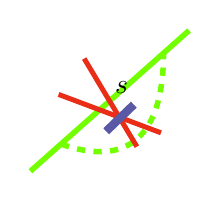
\begin{tikzpicture}[scale=.65]
\draw[green!55!yellow,line width=2pt](-1.6,-1.2)--(1.5,1.55);
\draw[green!55!yellow,line width=2pt,dashed](-1,-.67)..controls(.5,-1.2)and(1.0,-.25)..(1,1.1);
\draw[red!65!brown,line width=1.8pt](-.55,1.0)--(.48,-.72);
\draw[red!65!brown,line width=1.8pt](-1.05,.3)--(.95,-.45);
\draw[blue!30!gray,line width=3pt](-.12,-.42)--(.42,.1);
\node[above]at(.18,.12){\(s\)};
\end{tikzpicture}}

% E: text|right middle, modified F|Soit F'
Soit \(F'\) \deleted{\unsure{la face fermée}} \unsure{modifiée} obtenue\inserted{\((F'\supset F)\)}. Alors le polygone relatif correspondant à \(F\) est \(\varphi(\delta'F)\), et \deleted{elle est} le système défini canoniquement est canoniquement \deleted{\unsure{représenté par}}\inserted{isomorphe à} \deleted{\(\unsure{F',F'_0}\)} \((F',F'\cap L)\).

\margin{\uline{NB} \uline{(pour j)} pour \deleted{\unsure{2 arêtes}} qu'\unsure{un} pt critique \(s\) intervienne i.e. \deleted{\(\unsure{\varphi}\)} une face \(F\) est sur le côté privilégié, il \deleted{suffit}\inserted{\unsure{faut}} que les branches de \(L\) passant par \(s\) se recoupent toutes en un autre point du bord de \(F\) (dans le cas contraire \deleted{\unsure{elles sont}} une moitié des \unsure{branches sur le} bord de \(F\) sont toutes distinctes et se prolongent (cf. \(F\) et \(F'\) ci-dessous).}
% E: drawing|diagonal middle, two adjacent faces|F F' s t t'_1 t'_2 t'_3
\figure{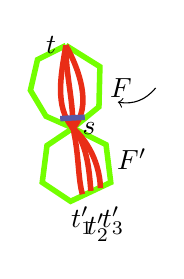
\begin{tikzpicture}[scale=.6]
\draw[green!55!yellow,line width=2pt](0,2)--(-.6,1.7)--(-.75,1.05)--(-.42,.5)--(.15,.25)--(.7,.7)--(.72,1.55)--(0,2);
\draw[green!55!yellow,line width=2pt](.15,.25)--(-.4,-.12)--(-.5,-.9)--(.1,-1.3)--(.95,-.9)--(.85,-.1)--(.15,.25);
\draw[red!65!brown,line width=2pt](0,2)..controls(-.1,1.4)and(-.25,.7)..(.15,.25)..controls(.28,-.3)and(.25,-.8)..(.35,-1.15);
\draw[red!65!brown,line width=2pt](0,2)..controls(.28,1.5)and(.57,.7)..(.15,.25)..controls(.65,-.2)and(.73,-.8)..(.73,-1.02);
\draw[red!65!brown,line width=2pt](0,2)..controls(.0,1.35)and(.15,.9)..(.15,.25)..controls(.48,-.1)and(.5,-.8)..(.53,-1.08);
\draw[blue!30!gray,line width=2pt](-.12,.45)--(.4,.48);
\node[left]at(0,2){\(t\)};\node[right]at(.15,.25){\(s\)};
\node[right]at(.73,1.1){\(F\)};\node[right]at(.88,-.4){\(F'\)};
\node[below]at(.35,-1.2){\(t'_1\)};\node[below]at(.68,-1.35){\(t'_2\)};\node[below]at(1,-1.2){\(t'_3\)};
\draw[->](1.9,1.1)to[bend left](1.1,.8);
\end{tikzpicture}}

% E: text|bottom right, k|Appelons un côté exceptionnel
k) Appelons un côté exceptionnel \uline{stable} ou instable (ou semi-stable) suivant que les deux \deleted{positions relatives} \inserted{\unsure{faces}} incidences correspondent à des p.r. stables (resp. instables) (condition \unsure{toujours} \unsure{top.}\unsure{ment} \unsure{forcée}). Nous \unsure{prendrons} le \unsure{sommet} exceptionnel le bord privilégié de la branche ord. de \(K\) qui y passe et des côtés en \unsure{bouts} exc. instables (\unsure{non forcé}).
\mspage{45}
\scanpage{47}
% E: text|upper left, l|Loi de symétrie
l) Loi de symétrie autour d'un côté exceptionnel (\unsure{y compris un côté fermé}), et structure locale autour d'une composante exceptionnelle de \(K\)

% E: drawing|left centre, long coloured configuration|six green transversals and red curves
\figure{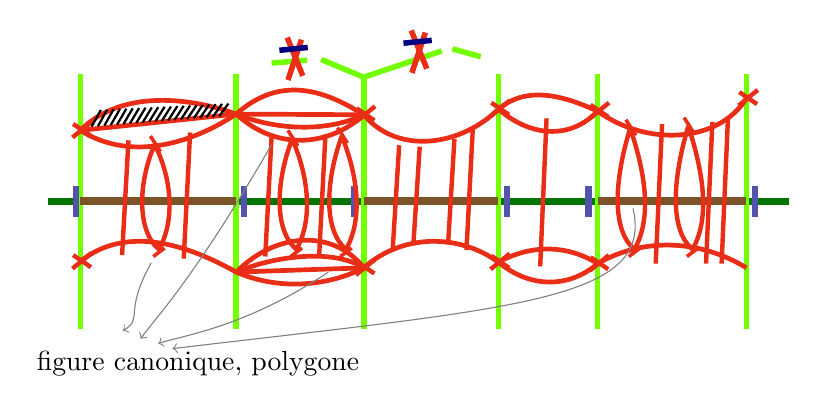
\begin{tikzpicture}[x=.9cm,y=.9cm]
\draw[green!45!black,line width=2.4pt](-.45,0)--(10,0);
\foreach \x in {0,2.2,4,5.9,7.3,9.4}{\draw[green!55!yellow,line width=2pt](\x,-1.8)--(\x,1.8);}
\foreach \a/\b in {0/2.2,4/5.9,7.3/9.4}{\draw[brown!65!black,line width=3pt](\a,0)--(\b,0);}
\foreach \x in {-.06,2.31,3.87,6.02,7.17,9.52}{\draw[blue!35!gray,line width=2.3pt](\x,-.22)--(\x,.22);}
\draw[red!65!brown,line width=1.7pt](0,1)..controls(.6,1.6)and(1.6,1.45)..(2.2,1.23)..controls(2.8,1.76)and(3.4,1.6)..(4,1.22)..controls(4.5,.63)and(5.4,.8)..(5.9,1.3)..controls(6.3,1.63)and(6.8,1.5)..(7.3,1.27)..controls(8,.77)and(9,.82)..(9.4,1.45);
\draw[red!65!brown,line width=1.7pt](0,1)..controls(.7,.56)and(1.55,.8)..(2.2,1.23)..controls(2.8,.68)and(3.55,.8)..(4,1.22);
\draw[red!65!brown,line width=1.7pt](0,1)--(2.2,1.23)--(4,1.22);
\draw[red!65!brown,line width=1.7pt](2.2,1.23)..controls(2.8,.99)and(3.5,.98)..(4,1.22);
\draw[red!65!brown,line width=1.7pt](5.9,1.3)..controls(6.4,.87)and(6.95,.9)..(7.3,1.27);
\draw[red!65!brown,line width=1.7pt](0,-.85)..controls(.6,-.37)and(1.4,-.55)..(2.2,-1.0)..controls(2.8,-.4)and(3.6,-.42)..(4,-.94)..controls(4.55,-.45)and(5.35,-.46)..(5.9,-.86)..controls(6.4,-.59)and(6.9,-.63)..(7.3,-.88)..controls(8,-.48)and(8.8,-.57)..(9.4,-.94);
\draw[red!65!brown,line width=1.7pt](2.2,-1)..controls(2.9,-1.3)and(3.6,-1.15)..(4,-.94);
\draw[red!65!brown,line width=1.7pt](2.2,-1)..controls(2.8,-.75)and(3.6,-.68)..(4,-.94);
\draw[red!65!brown,line width=1.7pt](2.2,-1)--(4,-.94);
\draw[red!65!brown,line width=1.7pt](5.9,-.86)..controls(6.4,-1.27)and(6.95,-1.19)..(7.3,-.88);
\foreach \x/\u/\v in {.68/.86/-.76,1.55/.97/-.81,2.7/.92/-.78,3.46/.94/-.78,4.5/.79/-.66,4.79/.77/-.62,5.28/.88/-.61,5.54/1.04/-.69,6.58/1.17/-.92,8.21/1.09/-.88,8.92/1.12/-.88,9.14/1.18/-.88}{\draw[red!65!brown,line width=1.6pt](\x,\u)--(\x-.09,\v);}
\foreach \x/\y in {1.05/.8,2.99/.88,3.69/.92,7.76/1.03,8.58/1.06}{\draw[red!65!brown,line width=1.6pt](\x,\y)..controls(\x-.24,.25)and(\x-.25,-.42)..(\x+.06,-.68)..controls(\x+.3,-.25)and(\x+.23,.35)..(\x,\y);\draw[red!65!brown,line width=1.3pt](\x-.06,\y+.12)--(\x+.08,\y-.1);\draw[red!65!brown,line width=1.3pt](\x-.02,-.78)--(\x+.14,-.66);}
\foreach \x/\y in {0/1,0/-.85,4/1.22,4/-.94,5.9/1.3,5.9/-.86,7.3/1.27,7.3/-.88,9.4/1.45}{\draw[red!65!brown,line width=1.6pt](\x-.11,\y-.1)--(\x+.16,\y+.12);\draw[red!65!brown,line width=1.6pt](\x-.1,\y+.09)--(\x+.15,\y-.08);}
\foreach \x in {.16,.25,.34,.43,.52,.61,.7,.79,.88,.97,1.06,1.15,1.24,1.33,1.42,1.51,1.60,1.69,1.78,1.87,1.96}{\draw[black,line width=.8pt](\x,1.04+\x*.08)--(\x+.13,1.28+\x*.05);}
\draw[green!55!yellow,line width=2pt](2.7,1.95)--(3.2,1.99);\draw[green!55!yellow,line width=2pt](3.4,2)--(4,1.75)--(5.1,2.12);\draw[green!55!yellow,line width=2pt](5.25,2.15)--(5.65,2.04);
\foreach \x/\y in {3/2.07,4.75/2.17}{\draw[red!65!brown,line width=2pt](\x-.08,\y+.24)--(\x+.14,\y-.3);\draw[red!65!brown,line width=2pt](\x+.12,\y+.21)--(\x-.07,\y-.36);\draw[blue!50!black,line width=2pt](\x-.19,\y+.06)--(\x+.21,\y+.1);}
\draw[gray,->](1,-.87)..controls(.6,-1.6)and(.9,-1.64)..(.6,-1.83);
\draw[gray,->](2.7,.8)..controls(1.6,-1.1)and(1.1,-1.6)..(.85,-1.94);
\draw[gray,->](3.5,-1)..controls(2.3,-1.8)and(1.4,-1.9)..(1.1,-2.01);
\draw[gray,->](7.8,-.1)..controls(8.1,-1.4)and(6.2,-1.5)..(1.3,-2.08);
\node[below right]at(-.75,-1.98){figure \unsure{canonique}, \deleted{\unsure{polygone}}};
\end{tikzpicture}}
\margin{\deleted{\unsure{voir}} i) j) ---}

% E: text|left below drawing, m|Indexation des sections
m) Indexation des sections de \(L\) sur les faces de \((X,K)\) \deleted{à l'aide de} par \(\widetilde I\), et passage d'une indexation à l'indexation de la face adjacente.

% E: text|lower left, n|Reconstitution de
n) Reconstitution de \deleted{\(\unsure{\xi}\)} \(\underline\Sigma\) (via \(\widetilde I\) ---) à l'aide de \(K\), et des constantes numériques associés à \(K\) (indices des sommets de \(K\)\inserted{\(\unsure{i(s)}\in\unsure{\frac12\mathbb Z|\frac12\mathbf Z}\) et \(\nu(s)\in\mathbb N\)}\inserted{\unsure{noté}}, \(\nu(a)\) des arêtes de \(K\)\deleted{\unsure{antiques}} \deleted{\(\unsure{\varphi}\)} (distinguons le cas des côtés ord\unsure{res} et des côtés exceptionnels.) Cf. aussi

\margin{\uline{NB} l'indice de chaque côté exceptionnel stable est \(\unsure{=|\geq}n-(\nu_s-1)-(\nu_t-1)\)\deleted{\(\unsure{\leq n}\)} et les instables \(\unsure{=|\geq}n-\nu\), où \(\nu\) est la multiplicité du sommet --- et la figure ci-contre est correcte ! On voit que l'indice des arêtes exceptionnelles résulte des autres données numériques.}

% E: text|right upper, NB|Il y a évidemment
\uline{NB} Il y a évidemment une loi de symétrie autour d'un côté ordinaire, pour ce qui est de la configuration induite par \(L\) sur les 2 faces adjacentes, au voisinage de l'arête en question. Peut-être $=$ \unsure{ceci est induit} : Considérer le couple \((X,K\cup L)\), et ``le voisinage ``tubulaire'' \unsure{standart}'' \(\overline T\) (\unsure{réunion d'``étoiles''}), du \deleted{\(K\) des côtés}\inserted{sous-complexe \(K\) de} \(K\cup L\) des arêtes \unsure{criti.} \deleted{\unsure{ordinaires}}. Alors pour toute arête \(a\) de \(K\), posant

% E: drawing|right centre, local crossing and curved edges|green T and red configuration
\figure{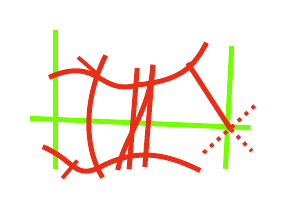
\begin{tikzpicture}[scale=.8]
\draw[green!55!yellow,line width=1.8pt](-.4,0)--(3.1,-.15);\draw[green!55!yellow,line width=1.8pt](0,-.8)--(0,1.4);\draw[green!55!yellow,line width=1.8pt](2.7,-.8)--(2.8,1.15);
\draw[red!65!brown,line width=1.8pt](-.1,.65)..controls(.7,1)and(.7,.35)..(1.3,.53)..controls(2,.6)and(2.2,.82)..(2.4,1.2);
\draw[red!65!brown,line width=1.8pt](-.2,-.45)..controls(.3,-.66)and(.3,-.97)..(.7,-.78)..controls(1.3,-.45)and(1.8,-.58)..(2.3,-.83);
\draw[red!65!brown,line width=1.8pt](.8,1)..controls(.4,.2)and(.5,-.55)..(.75,-.94);
\draw[red!65!brown,line width=1.8pt](1.3,.8)--(1.17,-.81);\draw[red!65!brown,line width=1.8pt](1.55,.85)--(1.42,-.77);
\draw[red!65!brown,line width=1.8pt](1.55,.85)..controls(1.5,.1)and(1.1,-.28)..(.99,-.82);
\draw[red!65!brown,line width=1.8pt](2.1,.88)--(2.78,-.17);\draw[red!65!brown,line width=1.4pt,dotted](2.35,-.55)--(3.22,.25);\draw[red!65!brown,line width=1.4pt,dotted](2.78,-.17)--(3.12,-.52);
\draw[red!65!brown,line width=1.4pt](.36,.97)--(.67,.7);\draw[red!65!brown,line width=1.4pt](.11,-.95)--(.35,-.67);
\end{tikzpicture}}

% E: display|right lower, definition T_a|T_a definition
\[
\overline T_a\overset{\mathrm{def}}=(F'\cup F'')\cap\overline T,
\]
% E: text|right lower, after T_a|F' F'' sont
\(F',F''\) sont les deux faces de \((\unsure{X},K)\) incidentes à \(a\); on a une involution \deleted{\(\unsure{\varphi}\)} \(\sigma_a\) de \(\unsure{a|\overline T_a}\), \unsure{ayant} \(a\) comme lieu de pts fixes, et qui \unsure{respecte} la structure \unsure{cellulaire} induite par \((X,K\cup L,\underline{\unsure{D}}\) \unsure{plus}, \deleted{\unsure{si \(a\) et \(b\)}} deux incidents au $=$ sommet \(s\), alors \(\sigma_a|\overline T_a\cap\overline T_b\) et \(\sigma_b|\overline T_a\cap\overline T_b\) \unsure{commutent les uns aux autres}.
\mspage{46}
\scanpage{48}
% E: text|upper left date|7.2.1984
\unsure{7.2.1984}
% E: text|upper left heading and paragraph|Structure de K
\uline{Structure de \(K\)}. \unsure{En y portant} des sommets d'ordre 2, soit \(S_K\) l'ens des sommets. On désigne par \(K\) le graphe top. \unsure{avec ces nouveaux sommets} (les anciens sont ceux de l'ordre 4). On a
% E: display|upper left, partition of vertices|S_K = S'_K union S''_K
\[
S_K=\underbrace{S'_K}_{\text{sommets rouges}}\sqcup
\underbrace{S''_K}_{\substack{\text{sommets}\ \deleted{\text{\unsure{rouges}}}\inserted{\text{noirs}}}}
\]
\margin{\uline{NB} \deleted{\unsure{\(S'_K\), \(S''_K\) sont}}\inserted{\(S'_K\) contient des} sommets d'ordre 2, \unsure{pas néc.|puis aussi} des sommets d'ordre 4. \(S''_K\) contient des sommets d'ordre 2, pas \unsure{néc.} d'ordre 4.}

% E: text|left middle, a|avec a) Pour tte face
avec :

a) Pour tte \deleted{\unsure{une}} face \(F\), \(S'_K\cap F\) et \(S''_K\cap F\) sont des subdivisions de \(\unsure{\delta F}\) \unsure{duales|doubles} l'une de l'autre, d'ordre \(2n\).

% E: text|left middle, NB|Deux sommets consécutifs
\deleted{\unsure{b)}}\inserted{NB} --- Deux sommets consécutifs sur \(\delta F\) ne sont pas d'ordre 4, et plus précisément, \deleted{entre deux} sur un arc de \(\delta F\) joignant deux sommets d'ordre 4, il y a toujours au moins un sommet rouge d'ordre 2, (et $=$ deux si \(\Sigma\) n'est pas \deleted{\unsure{double}} de type \(\mathrm{II}_p\) et si on est sur une arête exceptionnelle) et au moins un sommet noir (\unsure{il n'en est}\unsure{bq} pas dans le cas qu'on vient de dire\dots)

% E: text|lower left, b|On a une sélection
b) \deleted{\unsure{Enfin}} On a une \unsure{sélection des faces des bords} pour le déploiement \(K'\) de \(K\). Ainsi, chaque arête \(a\) d'une face \inserted{\(F\)} est munie d'un signe \(\varepsilon_F(a)\) qui est \(\unsure{+1|\pm1}\) si le bord est du côté de \(F\), \(-1\) sinon : On a les règles

% E: display|right upper, three sign rules|epsilon_F(a)
\[
\left\{\begin{array}{ll}
\varepsilon_F(a)=-\varepsilon_{F'}(a)&\text{si \(F,F'\) sont les deux faces incidentes à \(a\)}\\[6pt]
\varepsilon_F(\unsure{a})=\varepsilon_F(\unsure{b})&\begin{array}{l}\text{si \(a\) et \(b\) sont adjacentes}\\\text{sur \(F\), le sommet commun étant}\\\text{d'ordre 2}\end{array}\\[6pt]
\varepsilon_{a_1}(F_1)=\varepsilon_{a_2}(F_2)&\begin{array}{l}\text{si \(F_1\) et \(F_2\) sont adjacentes le long d'une}\\\text{arête quelconque \(b\), d'extrémité \(s\), d'ordre 4}\\\text{et que \(a_1\) et \(a_2\) sont incidentes à \(F_1\) et \(F_2\)}\\\text{resp., autres que \(b\), et incidentes à \(s\).}\end{array}
\end{array}\right.
\]
% E: drawing|right upper-middle below sign rules|b s cross
\figure{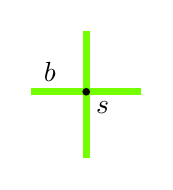
\begin{tikzpicture}[scale=.7]
\draw[green!55!yellow,line width=2.5pt](-1,0)--(1,0);\draw[green!55!yellow,line width=2.5pt](0,-1.2)--(0,1.1);
\fill(0,0)circle(2pt);\node[above]at(-.66,0){\(b\)};\node[below right]at(0,0){\(s\)};
\end{tikzpicture}}

% E: text|right middle, consequence|Il résulte du fait
Il résulte du fait que ttes les faces sont du $=$ ordre \(4n\), que pour \deleted{\unsure{chacune}} toute arête \(a\), si \(F,F'\) sont les deux faces incidentes, on a une donnée de \uline{symétrie autour de \(a\)}
% E: diagram|right middle, polygon isomorphism|sigma_a Pol(F) Pol(F')
\diagram{\begin{tikzcd}
\sigma_a^F\unsure{\simeq}\sigma_a:\ \deleted{\unsure{P}}\operatorname{Pol}(F)\arrow[r,"\sim"]&\operatorname{Pol}(F')
\end{tikzcd}}
\margin{\uline{NB} On a \(\sigma_a^F\sigma_a^{F'}=\mathrm{id}\).}
% E: text|right lower, characterization|caractérisé par la condition
\unsure{caractérisé par la condition de laisser} \deleted{invariantes}\inserted{fixes} les deux extrémités de \(a\). Il laisse donc \deleted{invariants}\inserted{fixes} \deleted{\unsure{tous}} tous les sommets et arêtes qui sont sur le ``grand côté'' \(\widehat a\) contenant \(a\) (bordé par les sommets d'ordre 4 les plus proches) (mais \deleted{\unsure{pas tous les pts}}\inserted{les prochains sommets} de part et d'autre de \(\widehat a\) sont non fixés par \(\sigma_a\)). L'application \(\sigma_a\) transforme sommets rouges (resp. noirs) en sommets noirs
\margin{\uline{NB} \(\sigma_a^F=\unsure{\sigma_{a'}^F|\sigma_a^{F'}}\) \unsure{si \(a,a'\) sont sur le $=$} \uline{\unsure{gd côté}}.}
\mspage{47}
\scanpage{49}
% E: text|upper left date|2.1.84
2.1.84
% E: text|upper left, cancelled draft opening|On place sur K
\deleted{On place sur \(K\) des nouveaux sommets (d'ordre 2), de la façon suivante; \deleted{Pour \unsure{chaque face (soit \(F\)) du quadrillage, on prend les sommets}} \unsure{points par côté fermé}.

% E: text|upper left, cancelled a and b|On rajoute les pts
\deleted{a) On rajoute les pts de \(K\cap L\) sur \(\delta F\).

b) Pour toute arête du nouveau complexe topologique \((\delta F,S\cap\unsure{\partial F|\delta F}\cup(\delta F\cap L))\), \unsure{on en distingue}}

% E: drawing|left upper-middle, marked edge|s and red orange marks
\figure{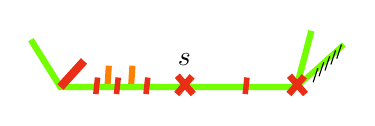
\begin{tikzpicture}[scale=.75]
\draw[green!55!yellow,line width=2.3pt](-.5,.8)--(0,0)--(4,0)--(4.25,.95);\draw[green!55!yellow,line width=2pt](4,0)--(4.8,.72);
\draw[red!65!brown,line width=3pt](0,0)--(.4,.44);
\foreach \x in {.6,.95,1.45,3.13}{\draw[red!65!brown,line width=2pt](\x,-.12)--(\x+.03,.16);}
\foreach \x in {.8,1.2}{\draw[orange,line width=2.2pt](\x,.05)--(\x+.02,.36);}
\foreach \x in {2.1,4}{\draw[red!65!brown,line width=2.4pt](\x-.13,-.12)--(\x+.13,.18);\draw[red!65!brown,line width=2.4pt](\x-.12,.19)--(\x+.15,-.12);}
\node[above]at(2.1,.2){\(s\)};
\foreach \x in {4.28,4.38,4.48,4.58,4.68}{\draw[black](\x,\x-4.2)--(\x+.08,\x-3.96);}
\end{tikzpicture}}

% E: text|upper middle, replacement a|Rajoutons les pts
a) Rajoutons les pts de \(\widehat a\cap L\)
% E: display|upper middle|a' = (a,a intersect S(K) union a intersect L)
\[
-\quad\text{soit }\underline{a}'=(a,a\cap S(K)\cup a\cap L)
\]
% E: text|middle left, structure and NB|Le graphe
\unsure{Le graphe est ainsi structuré}\inserted{top.}, soit \(\alpha\) une arête de ce graphe. (\uline{NB} \deleted{\(\unsure{\xi}\)} Il y a au moins un \deleted{c) Si une des est} élément de \(a\cap L\) (``\deleted{\unsure{arête}}\inserted{sommet} rouge'') sur \(a\) distinct des extrémités, donc chaque arête \(\alpha\) de \(\underline a'\) \deleted{est} a au moins une extrémité rouge, i.e. qui n'est pas une \deleted{sommet}\inserted{extrémité} de \(\underline a\), et il y en a exactement deux qui n'en ont qu'une de rouge (\unsure{c'est les ptés arêtes}).

% E: text|lower left, new a|Sur ces dernières
a) Sur ces dernières, on ne rajoute pas d'autre sommet\inserted{\unsure{sauf si l'extrémité est un sommet de \(L\)}}. \deleted{Sur toutes}\inserted{\unsure{Pour les}} autres arêtes, on \deleted{\unsure{dis}} rajoute des sommets (oranges) de la façon suivante

% E: text|lower left, b|Si les deux extrémités
b) Si \deleted{\unsure{ttes}} les\inserted{deux} extrémités sont non critiques, i.e. ne sont pas des sommets de \(\unsure{L|K}\), on rajoute juste un sommet (le milieu)

% E: text|bottom left, c unfinished|Pour les deux autres arêtes
c) \deleted{Sinon} Pour les deux autres arêtes (cas d'une arête \(\underline a\) ordinaire), de part et d'autre du pt critique \deleted{\(\unsure{\xi}\)} \(s\), si \(\nu(s)\) est un \unsure{ordre|entier}, on dispose \(\frac{\nu(s)}2\) pts \unsure{oranges|rouges} (si
}

% E: drawing|upper right, isolated green angle with red vertex and tick|green angle red cross
\figure{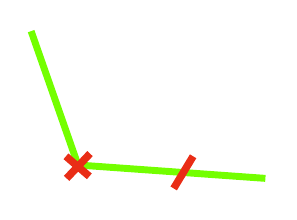
\begin{tikzpicture}[scale=.85]
\draw[green!55!yellow,line width=2.5pt](-.7,2)--(0,0)--(2.8,-.2);
\draw[red!65!brown,line width=2.7pt](-.17,-.2)--(.18,.17);\draw[red!65!brown,line width=2.7pt](-.18,.13)--(.17,-.17);
\draw[red!65!brown,line width=2.7pt](1.43,-.35)--(1.72,.13);
\end{tikzpicture}}
\mspage{48}
\scanpage{50}
% E: text|upper left, question|J'aimerais comprendre
J'aimerais comprendre la relation entre les \(\sigma_a^F\), et les \uline{signes} \(\varepsilon_F(a)\).

% E: text|upper left, transition|Mais il faut encore
Mais il faut encore introduire une autre structure.

% E: text|left upper-middle, c|Ensemble C_K
c) Ensemble \(C_K\unsure{\subset|\in}S_K\) des ``pts critiques''\inserted{ils sont d'ordre 2, \unsure{tels que}}, avec la condition que sur chaque \deleted{\unsure{arc}} grand côté, il y a \deleted{\unsure{au plus}}\inserted{exactement} un \deleted{tel} élément de \(C_K\).

\deleted{(quand il n'y en a pas, l'arête est dite exceptionnelle)} De plus, chaque pt critique \(s\) est muni d'un poids \(\nu(s)\geq\unsure{2|1}\),\inserted{qui est pair ou impair, suivant que \(s\) est noir, ou rouge,} (le poids d'un élément de \(S_K\) est par définition \(\nu(s)\) si critique, 1 si non critique \deleted{\unsure{de poids}} et dans \(S'_K\), 0 s'il est non critique et est dans \(S''_K\)).

\margin{définir les ``arcs critiques'' ou ``arcs de transition'' d'amplitude totale sur les côtés, \(\nu(s)\) ou \unsure{encore} \(2\nu(s)\) (il contient \unsure{\(\nu(s)\) subdivisions} \deleted{de \(S_K\)}\inserted{\unsure{\(S_2\)}} \unsure{et sommets rouges}).}
\margin{Les pts critiques sont des centres des \unsure{arcs critiques}, et déterminent les indices (\unsure{comme la moitié de l'amplitude des arcs critiques dans le cas}) --- \unsure{les voisins des sommets sur ces arcs sont non critiques}.}
\margin{\uline{NB} Les arcs de transition (fermés) sont mutuellement disjoints.}
\margin{Les sommets d'ordre 4 sont exactement \deleted{\unsure{ceux qui sont les}} les \unsure{milieux des arcs} \deleted{\unsure{antipodiques}}\inserted{critiques} \deleted{\unsure{\(\forall\) les arcs antipodiques}}.}

% E: text|left lower-middle, introduction|En termes des sommets critiques
En termes des sommets critiques, on a ceci :

% E: text|left lower, 1|Soit s un sommet critique
1) Soit \(s\) un sommet critique, incident à la face \(F\). Soit \(s'\) son antipodique dans \(\delta F\). \deleted{Alors si \(s'\) est aussi critique, \unsure{on doit le signe \(\varepsilon_a\)}}\inserted{Pour qu'on ait \(\varepsilon_F(a)=+1\), il f. et il s.} que les sommets\inserted{\(s'\)} antipodiques de \(s\)\inserted{\unsure{critiques}} soient également critiques (il a alors le $=$ indice).
\margin{relation entre \(C_K\) et les signes \(\varepsilon_F(a)\)}

% E: text|bottom left, 2 unfinished|Pour toute face F
2) Pour tte face \(F\), il y a au moins 3 pts critiques sur \(\delta F\) (et $=$ au moins 4, \deleted{\unsure{3q si tous les pts}} il y a au moins un pt critique\inserted{\(s\)} de signe \(+1\). \deleted{\unsure{Pour tout}} \unsure{cas, sur chacun}
\mspage{49}
\scanpage{51}
% E: text|upper left, date|2.1.84.
2.1.84.

\deleted{
% E: text|left upper, introduction|On place sur K
On place sur \deleted{\unsure{un graphe}} \(K\) deux ensembles de pts, \(S'_K\ S''_K\) \deleted{\unsure{et}}, de telle façon que
\inserted{\(S'_K\) : sommets rouges ; \(S''_K\) : sommets \unsure{oranges}}

% E: text|left upper, bracketed paragraph|pour toute face
\deleted{\unsure{b)}} \(\forall\ F\) face de \(K\), \(\delta F\cap S'\) est un polygone top. d'ordre \(2n\), et sur chaque côté \inserted{\(\alpha\)} de celui-ci il y a un pt de \(S''\) et un seul, qui est son milieu si \(\alpha\) est \unsure{entier|ordinaire}.

\deleted{a) \(\unsure{S'_K\subset L}\) \unsure{tous les sommets}}
\deleted{a) \(\unsure{S(K)\cap S'_K\supset K\cap L\setminus K\cap S(L)}\)}

% E: display|left middle, a|S'_K intersection L
a) \(S'_K\cap L=K\cap L\setminus(\text{ensemble des pts critiques de }K\text{ qui sont d'ordre impair})\)

\deleted{b) \(S'_K\cap S(K)=S(K)\cap L\)}

% E: text|left middle, b|Pour toute arête
b) \deleted{\unsure{Ensuite}} Pour toute arête (ord.) \(a\) de \(K\), on a \(a\cap S'_K\ne\varnothing\). \inserted{\unsure{des vrais côtés de \(K\),}} et l'unique sommet de \(K\) sur \(\alpha\) dans les cas ci-contre.

% E: drawing|left middle, small crossed segment|green segment red and orange marks
\figure{
\begin{tikzpicture}[scale=.7]
\draw[yellow!60!green,line width=2pt] (0,0)--(2.1,0);
\draw[red!70!black,line width=2pt] (.8,-.13)--(.8,.13) (1.2,-.13)--(1.2,.13);
\draw[orange,line width=3pt] (1,-.12)--(1,.12);
\draw[black,line width=1pt] (-.05,.02)--(.2,.18)--(.06,.08)--(.5,.12)--(.7,.1)--(1.4,.18)--(1.65,.13)--(2.2,.2);
\end{tikzpicture}}

% E: drawing|left middle, lower segment|dotted green segment red centre
\figure{
\begin{tikzpicture}[scale=.8]
\draw[yellow!60!green,line width=2pt,densely dotted] (0,0)--(3.2,.1);
\fill[yellow!60!green] (0,0) circle(.09) (3.2,.1) circle(.09);
\draw[red!70!black,line width=3pt] (1.2,.04)--(2,.07);
\draw[orange,line width=3pt] (1.6,-.17)--(1.6,.27);
\end{tikzpicture}}

% E: drawing|left middle, small angle|green angle orange corner
\figure{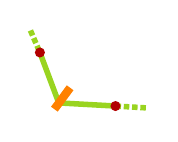
\begin{tikzpicture}[scale=.8]
\draw[yellow!60!green,line width=2pt] (0,1)--(.3,.2)--(1.2,.15);
\draw[yellow!60!green,line width=2pt,densely dotted] (-.15,1.35)--(0,1) (1.2,.15)--(1.7,.12);
\fill[red!70!black] (0,1) circle(.08) (1.2,.15) circle(.08);
\draw[orange,line width=3pt] (.23,.1)--(.48,.44);
\end{tikzpicture}}

% E: text|left lower, NB|a et b impliquent
\uline{NB} a) et b) impliquent que \(S'_K\cap S(K)=S(K)\cap L\), i.e. un sommet de \(K\) est dans \(S'_K\) ssi il est dans \(L\).

% E: text|left bottom, c|Pour tt pt critique
c) Pour tt pt critique \(s\) de \(K\), sur l'arête
\deleted{\(S'_K\setminus S_K\cap L\) est réunion de segments, \unsure{en plus de quelques pts isolés de \(K\) qui}}
désignons par \(t',t''\) les pts les plus proches de \(s\), sur l'arête \(a\) de \(K\) contenant \(s\), parmi les pts de \((a\cap L)\unsure{\cap|\cup}\partial a\).
L'intersection \([t',t'']\cap S'_K\) est de cardinal égal :
\deleted{\unsure{on disposera sur le segment \([t',t'']\)}}
\(\nu(s)\), \deleted{et il y a \unsure{un}}
}

% E: drawing|right top|oval thick boundary arcs crossing curves
\figure{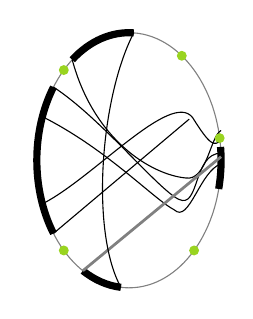
\begin{tikzpicture}[x=1cm,y=1cm,scale=.9]
\draw[gray] (0,0) ellipse (1.3 and 1.8);
\draw[line width=2.6pt] (87:1.3 and 1.8) arc(87:128:1.3 and 1.8) (145:1.3 and 1.8) arc(145:215:1.3 and 1.8) (240:1.3 and 1.8) arc(240:265:1.3 and 1.8) (-13:1.3 and 1.8) arc(-13:6:1.3 and 1.8);
\draw (145:1.3 and 1.8) .. controls (-.4,.6) and (.4,-.4) .. (.7,-.55) .. controls (1,-.7) and (.9,.1) .. (1.3,.1);
\draw (128:1.3 and 1.8) .. controls (-.5,.3) and (.3,-.2) .. (.8,-.25) .. controls (1.1,-.3) and (1.15,.35) .. (1.3,.42);
\draw (160:1.3 and 1.8) .. controls (-.3,.15) and (.35,-.55) .. (.64,-.7) .. controls (.85,-.9) and (1,-.15) .. (1.3,-.05);
\draw (200:1.3 and 1.8) .. controls (-.5,-.25) and (.6,1) .. (.9,.6) .. controls (1.15,.2) and (1.2,.2) .. (1.3,.28);
\draw (215:1.3 and 1.8)--(.85,.58);
\draw[gray,line width=1pt] (240:1.3 and 1.8)--(1.3,.05);
\draw (265:1.3 and 1.8) .. controls (-.55,-1) and (-.4,.9) .. (87:1.3 and 1.8);
\foreach \a in {135,55,10,225,315}{\fill[yellow!60!green] (\a:1.3 and 1.8) circle(.07);}
\end{tikzpicture}}

% E: drawing|right middle left|red hexagon central orange point green arrows
\figure{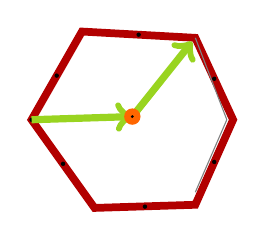
\begin{tikzpicture}[scale=.8]
\draw[red!70!black,line width=2.8pt] (0,1.5)--(.8,2.9)--(2.6,2.8)--(3.2,1.5)--(2.6,.15)--(1,.1)--cycle;
\foreach \p in {(0,1.5),(.4,2.2),(1.7,2.85),(2.9,2.15),(2.9,.83),(1.8,.12),(.5,.8)}{\fill \p circle(.035);}
\draw[yellow!60!green,line width=2.6pt,->] (0,1.5)--(1.6,1.55);
\draw[yellow!60!green,line width=2.6pt,->] (1.6,1.55)--(2.55,2.74);
\fill[orange!80!red] (1.6,1.55) circle(.13);
\fill[black] (1.6,1.55) circle(.025);
\draw[gray] (2.6,2.8)--(3.1,1.5)--(2.6,.35);
\end{tikzpicture}}

% E: drawing|right middle right|red pentagon green straight passage
\figure{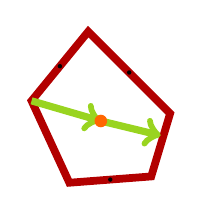
\begin{tikzpicture}[scale=.8]
\draw[red!70!black,line width=2.8pt] (0,1.3)--(.9,2.4)--(2.2,1.1)--(1.9,.1)--(.6,0)--cycle;
\foreach \p in {(.45,1.85),(1.55,1.75),(1.25,.05)}{\fill \p circle(.035);}
\draw[yellow!60!green,line width=2.6pt,->] (0,1.3)--(1.1,.98);
\draw[yellow!60!green,line width=2.6pt,->] (1.1,.98)--(2.05,.75);
\fill[orange!80!red] (1.1,.98) circle(.1);
\end{tikzpicture}}

% E: drawing|right lower middle|broken red polygon green bent arrows pencil lines
\figure{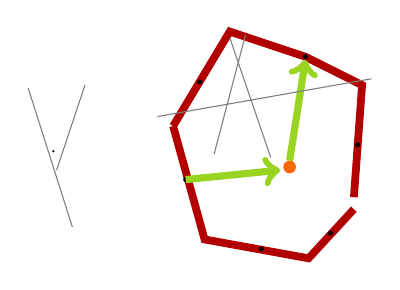
\begin{tikzpicture}[scale=.8]
\draw[red!70!black,line width=2.8pt] (0,1.8)--(.9,3.3)--(2.1,2.9)--(3,2.45)--(2.87,.67) (2.87,.48)--(2.15,-.3)--(.5,0)--(0,1.8);
\foreach \p in {(.42,2.5),(2.1,2.9),(2.93,1.5),(2.5,.1),(1.4,-.15),(.2,.95)}{\fill \p circle(.04);}
\draw[yellow!60!green,line width=2.6pt,->] (.2,.95)--(1.7,1.1);
\draw[yellow!60!green,line width=2.6pt,->] (1.85,1.25)--(2.1,2.85);
\fill[orange!80!red] (1.85,1.15) circle(.1);
\draw[gray] (-.25,1.95)--(3.15,2.55) (.9,3.2)--(1.55,1.3) (1.15,3.25)--(.65,1.35);
\draw[gray] (-2.3,2.4)--(-1.6,.2) (-1.4,2.45)--(-1.85,1.1);
\fill (-1.9,1.4) circle(.02);
\end{tikzpicture}}

% E: drawing|right bottom right|three red crossing branches green passage
\figure{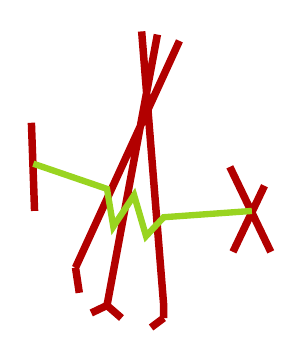
\begin{tikzpicture}[scale=.8]
\draw[red!70!black,line width=2.7pt] (0,.6)--(1.65,4.2) (0,.6)--(.06,.2) (.5,0)--(1.3,4.3) (.25,-.12)--(.5,0)--(.73,-.2) (1.4,-.2)--(1.4,0)--(1.05,4.35) (1.4,-.2)--(1.2,-.35) (-.65,1.5)--(-.7,2.9) (2.5,.85)--(3,1.9) (2.45,2.2)--(3.1,.85);
\draw[yellow!60!green,line width=2.3pt] (-.67,2.25)--(.5,1.85)--(.6,1.25)--(.93,1.75)--(1.12,1.1)--(1.4,1.4)--(2.8,1.5);
\end{tikzpicture}}

% E: drawing|right bottom left|red crossing graph green W and dotted segments
\figure{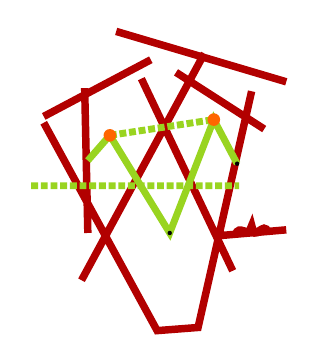
\begin{tikzpicture}[scale=.8]
\draw[red!70!black,line width=2.7pt] (0,3)--(1.8,-.3)--(2.45,-.25)--(3.3,3.5) (.6,.5)--(2.55,4.1) (.7,1.25)--(.65,3.55) (1.55,3.7)--(3,0.65) (0,3.1)--(1.7,4) (1.15,4.45)--(3.85,3.65) (2.1,3.8)--(3.5,2.9) (2.7,1.2)--(3.85,1.3);
\draw[yellow!60!green,line width=2.5pt] (.7,2.4)--(1.05,2.8)--(2,1.25)--(2.7,3.05)--(3.07,2.35);
\draw[yellow!60!green,line width=2.5pt,densely dotted] (1.05,2.8)--(2.7,3.05) (-.2,2)--(3.1,2);
\fill[orange!80!red] (1.05,2.8) circle(.1) (2.7,3.05) circle(.1);
\fill (2,1.25) circle(.035) (3.07,2.35) circle(.035);
\draw[red!70!black,line width=3pt] (3.05,1.22)..controls (3.1,1.4) and (3.25,1.15)..(3.3,1.35)..controls (3.35,1.1) and (3.5,1.45)..(3.55,1.26);
\end{tikzpicture}}
\mspage{50}
\scanpage{52}
% E: margin note|top, continuation|dans chacun des arcs
\margin{\deleted{\unsure{NB}} dans chacun des arcs \deleted{\unsure{complémentaires}} déterminés par \(s,t\) sur \(\delta F\), il y a au moins un pt critique.}

% E: text|left upper, d|Relation entre sommets critiques
d) \uline{Relation entre} sommets critiques \deleted{\unsure{de}} sur \(F\) et sur \(F'=\sigma_a(F)\)

\(a\) un \uline{grand côté} sur \(\delta F\). OPS que \(\varepsilon_F(a)=1\) (quitte à intervertir les rôles de \(F\) et \(F'\)). On a deux cas :

% E: text|left upper-middle, definitions|Soit t l'antipodique
Soit \deleted{\unsure{\(s\) le pt critique sur \(a\)}}\inserted{\(t\) l'antipodique de \(s\), qui est critique}, \(u,v\) les deux pts critiques les plus voisins de \unsure{\(t\)|\(s\)} \deleted{de \(\delta F\)} de part et d'autre de \(s\), \(\beta=\widehat{\unsure{u^*tv^*|utv}}\) l'arc correspondant\inserted{de \(\delta F\)}, d'extrémités \(u,v\) contenant \(s\). Considérons \unsure{\(\beta\)}\inserted{l'autre} arc d'extrémités \(\unsure{u^*|u}\) et \(v^*\), soit \(\alpha\). \deleted{Soit} (NB, on a \(u,v\) sur deux arcs\inserted{ouverts} distincts déterminés par \(s,t\) sur \(\delta F\), \deleted{\unsure{et}} et \(u\ne v\), donc \unsure{\(s\in\)}\deleted{\(\beta\)}\inserted{\(\alpha\)}, de façon précise \(\alpha=\widehat{usv}\)). \deleted{\unsure{Donnons}} \(\unsure{s'=s},t',u',v'\) \deleted{\unsure{les}} transformés de \(s,t,u,v\) par \(\sigma_a\).

% E: drawing|left middle|two tangent ovals s t u v and primes
\figure{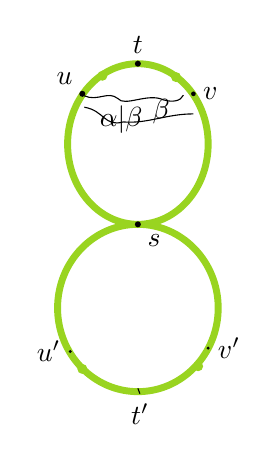
\begin{tikzpicture}[scale=.85]
\draw[yellow!60!green,line width=2.5pt] (0,1.25) ellipse (1.05 and 1.2) (0,-1.2) ellipse (1.2 and 1.25);
\fill (0,.05) circle(.045) node[below right] {$s$};
\fill (0,2.45) circle(.045) node[above] {$t$};
\fill (-.83,2) circle(.045) node[above left] {$u$};
\fill (.83,2) circle(.035) node[right] {$v$};
\fill (-1.01,-1.85) circle(.025) node[left] {$u'$};
\fill (1.05,-1.8) circle(.025) node[right] {$v'$};
\draw (0,-2.4)--(.03,-2.48) node[below] {$t'$};
\foreach \p in {(-.53,2.27),(.57,2.25),(-.83,-2.11),(.9,-2.07)}{\fill[yellow!60!green] \p circle(.075);}
\draw (-.8,1.97)..controls (-.6,1.88) and (-.45,2.05)..(-.3,1.93)..controls (-.2,1.8) and (.15,2.02)..(.38,1.91)..controls (.52,1.87) and (.64,1.89)..(.68,1.98);
\node at (.35,1.74) {$\beta$};
\draw (-.8,1.8)..controls (-.5,1.75) and (-.5,1.5)..(-.22,1.58)..controls (.15,1.55) and (.42,1.7)..(.83,1.7);
\node at (-.25,1.61) {$\deleted{\unsure{\alpha|\beta}}$};
\end{tikzpicture}}

% E: text|left middle-lower, a|sigma induit une bijection
Alors

a) \deleted{\unsure{\(C_K\)}} \uline{\(\sigma_a\) induit une bijection entre \(C_K\cap\alpha\) et \(C_K\cap\alpha'\)}.
\deleted{\unsure{Jeux induits, avec la condition ci-dessous, que}}
Si \(x\) et \(x'\) se correspondent par \(\sigma_a\), on a \(\varepsilon_F(x)=\varepsilon_{\unsure{F|F'}}(x')\), sauf si \(x=s\), donc \(x'=s\) (auquel cas \(\varepsilon_{F'}(x)=-\varepsilon_F(x)\)).

% E: text|left lower, b|On a t' non critique
b) On a \(t'\notin C_K\), \deleted{l'intersection} \(\operatorname{card}(\mathring{\beta}'\cap C_K)\)\deleted{\unsure{\(\leq2\)}}\(\in\{0,1,2\}\).
\inserted{Donc si l'ordre\inserted{\unsure{réduit}} de \(F\) resp. \(F'\) est \(N\) resp. \(N'\), on a \(N'\in\{N-1,N,N+1\}\)}
\deleted{\unsure{tout à}} Si \(x\in\mathring{\beta}'\cap C_K\), on a \(\varepsilon_F(x)=-1\).

% E: text|left bottom, corollary|Considérons les antipodiques
\uline{Cor} Considérons les antipodiques \(u^*,v^*\) de \(u,v\) sur \(\delta F\), et l'arc \(\beta^*=\widehat{u^*sv^*}\), \deleted{Alors} \unsure{dans|alors} son intérieur il n'y a pas de pts critiques de signe \(\unsure{\ne1|+1}\).

% E: text|right top, summary|En résumé
\uline{En résumé} Soit \(x\in S_K\cap\delta F\), \deleted{\unsure{un sommet de \(s\)}} \(x'=\sigma_a(\unsure{F|x})\), alors \(x'\) est critique ssi \(x\) l'est, et \(x\) et \(x'\) ont $=$ indice sauf dans les cas suivants

% E: display|right upper, a|x equals s
a) \(x=s\), auquel cas : \(\varepsilon_{F'}(x)=-\varepsilon_F(x')\)

% E: text|right upper-middle, b|x equals t
b) \(x=t\), auquel cas \deleted{\unsure{un}} \(\unsure{x|t}\) est critique d'indice \(+1\), \(\unsure{x''|x'}\) non critique

% E: text|right middle, parenthesis|Ceci permet de distinguer
(Ceci permet de distinguer \deleted{\unsure{quel}}\inserted{lequel} des deux faces \(F,F'\) est ``\deleted{\unsure{principale}}\inserted{\uline{\unsure{privilégié}}}'' par rapport à l'autre, en termes de la position de l'unique critique \(\unsure{s}\) sur \(a\), et ses \deleted{\unsure{deux}} antipodiques sur \(\delta F,\delta F'\))

% E: text|right lower, c|x in open arc
c) \(x\in\mathring{\widehat{utv}}=\mathring{\beta}\), avec \(x\ne t\)

i.e. \(x'\ne t'\), alors \(x\) non critique, alors il peut exister 1 ou 2 cas (au maximum) tels que \(x'\) soit critique --- son indice est alors \(-1\).
\mspage{51}
\scanpage{53}
% E: text|printed header, upper left|//* CRAY2 0411 I
\texttt{//*\quad CRAY2\quad 0411\qquad I}

% E: drawing|printed upper banner|four zero characters formed from zeros
\figure{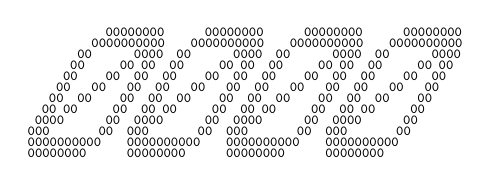
\begin{tikzpicture}[x=.09cm,y=.14cm,every node/.style={font=\tiny\ttfamily,anchor=west,inner sep=0pt}]
\foreach \d in {0,14,28,42}{
\node at ({\d+11},0) {00000000};
\node at ({\d+9},-1) {0000000000};
\node at ({\d+7},-2) {00}; \node at ({\d+15},-2) {0000};
\node at ({\d+6},-3) {00}; \node at ({\d+13},-3) {00}; \node at ({\d+16},-3) {00};
\node at ({\d+5},-4) {00}; \node at ({\d+11},-4) {00}; \node at ({\d+15},-4) {00};
\node at ({\d+4},-5) {00}; \node at ({\d+9},-5) {00}; \node at ({\d+14},-5) {00};
\node at ({\d+3},-6) {00}; \node at ({\d+7},-6) {00}; \node at ({\d+13},-6) {00};
\node at ({\d+2},-7) {00}; \node at ({\d+5},-7) {00}; \node at ({\d+12},-7) {00};
\node at ({\d+1},-8) {0000}; \node at ({\d+11},-8) {00};
\node at (\d,-9) {000}; \node at ({\d+10},-9) {00};
\node at (\d,-10) {0000000000};
\node at (\d,-11) {00000000};
}
\end{tikzpicture}}

% E: drawing|printed middle banner|CRAY2 formed from repeated characters
\figure{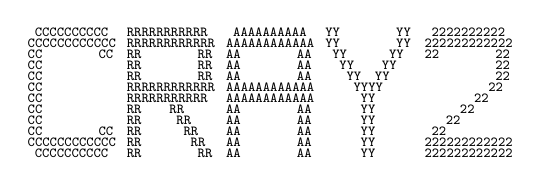
\begin{tikzpicture}[x=.09cm,y=.14cm,every node/.style={font=\tiny\ttfamily,anchor=west,inner sep=0pt}]
\node at (1,0) {CCCCCCCCCC}; \node at (0,-1) {CCCCCCCCCCCC};
\foreach \r in {2,3,4,5,6,7,8,9}{\node at (0,-\r) {CC};}
\node at (10,-2) {CC}; \node at (10,-9) {CC};
\node at (0,-10) {CCCCCCCCCCCC}; \node at (1,-11) {CCCCCCCCCC};
\node at (14,0) {RRRRRRRRRRR}; \node at (14,-1) {RRRRRRRRRRRR};
\foreach \r in {2,3,4,7,8,9,10,11}{\node at (14,-\r) {RR};}
\foreach \r in {2,3,4}{\node at (24,-\r) {RR};}
\node at (14,-5) {RRRRRRRRRRRR}; \node at (14,-6) {RRRRRRRRRRR};
\node at (20,-7) {RR}; \node at (21,-8) {RR}; \node at (22,-9) {RR}; \node at (23,-10) {RR}; \node at (24,-11) {RR};
\node at (29,0) {AAAAAAAAAA}; \node at (28,-1) {AAAAAAAAAAAA};
\foreach \r in {2,3,4,7,8,9,10,11}{\node at (28,-\r) {AA}; \node at (38,-\r) {AA};}
\node at (28,-5) {AAAAAAAAAAAA}; \node at (28,-6) {AAAAAAAAAAAA};
\foreach \r in {0,1}{\node at (42,-\r) {YY}; \node at (52,-\r) {YY};}
\node at (43,-2) {YY}; \node at (51,-2) {YY};
\node at (44,-3) {YY}; \node at (50,-3) {YY};
\node at (45,-4) {YY}; \node at (49,-4) {YY};
\node at (46,-5) {YYYY};
\foreach \r in {6,7,8,9,10,11}{\node at (47,-\r) {YY};}
\node at (57,0) {2222222222}; \node at (56,-1) {222222222222};
\node at (56,-2) {22}; \node at (66,-2) {22};
\node at (66,-3) {22}; \node at (66,-4) {22}; \node at (65,-5) {22}; \node at (63,-6) {22}; \node at (61,-7) {22}; \node at (59,-8) {22}; \node at (57,-9) {22};
\node at (56,-10) {222222222222}; \node at (56,-11) {222222222222};
\end{tikzpicture}}

% E: text|printed middle-lower, six repeated lines|START JOB 411 CRAY2
\texttt{****A\quad START\quad JOB\quad 411\quad CRAY2\qquad ROOM\qquad 4.18.41 PM 16 AUG 82\quad R6.PR1\quad SYS JES2\quad JOB 411\quad START\quad A****}\par
\texttt{****A\quad START\quad JOB\quad 411\quad CRAY2\qquad ROOM\qquad 4.18.41 PM 16 AUG 82\quad R6.PR1\quad SYS JES2\quad JOB 411\quad START\quad A****}\par
\texttt{****A\quad START\quad JOB\quad 411\quad CRAY2\qquad ROOM\qquad 4.18.41 PM 16 AUG 82\quad R6.PR1\quad SYS JES2\quad JOB 411\quad START\quad A****}\par
\texttt{****A\quad START\quad JOB\quad 411\quad CRAY2\qquad ROOM\qquad 4.18.41 PM 16 AUG 82\quad R6.PR1\quad SYS JES2\quad JOB 411\quad START\quad A****}\par
\texttt{****A\quad START\quad JOB\quad 411\quad CRAY2\qquad ROOM\qquad 4.18.41 PM 16 AUG 82\quad R6.PR1\quad SYS JES2\quad JOB 411\quad START\quad A****}\par
\texttt{****A\quad START\quad JOB\quad 411\quad CRAY2\qquad ROOM\qquad 4.18.41 PM 16 AUG 82\quad R6.PR1\quad SYS JES2\quad JOB 411\quad START\quad A****}

% E: text|printed lower left, notice header|DERNIERE MISE A JOUR
\texttt{DERNIERE MISE A JOUR DE JOURNAL : 11-08-82}\par
\texttt{ATTENTION ...........}

% E: text|printed lower left, notice 1|ARRET DE L'ORDINATEUR
\texttt{1. ARRET DE L'ORDINATEUR LE MARDI 17 AOUT DE 7 H A 8 H.}

% E: text|printed lower left, notice 2|UNE MODIFICATION SYSTEME
\texttt{1\qquad 2. UNE MODIFICATION SYSTEME NOUS CONTRAINDRA A DETRUIRE}\par
\texttt{1\qquad\phantom{2. }LE CONTENU DU DISQUE SPOOL LE MARDI 17 AOUT A 6 HEURES}\par
\texttt{1\qquad\phantom{2. }VEUILLEZ RECUPERER VOS SORTIES EN ATTENTE AVANT CETTE}\par
\texttt{1\qquad\phantom{2. }DATE. MERCI DE VOTRE COMPREHENSION.}

% E: text|printed lower left, notice 3|UN ARRET EXCEPTIONNEL
\texttt{1\qquad 3. UN ARRET EXCEPTIONNEL POUR PREPARER L'ARRIVEE DE NOUVELLES}\par
\texttt{1\qquad\phantom{3. }UNITES AURA LIEU DU VENDREDI 20 AOUT A 17H \unsure{30} AU LUNDI}\par
\texttt{1\qquad\phantom{3. }23 AOUT A 8H.}

% E: drawing|handwritten bottom left|red crossing green polygon black edges
% E: drawing|handwritten bottom right|red crossing green polygon dashed chord
% E: drawing|handwritten bottom centre|long red separating curve
\figure{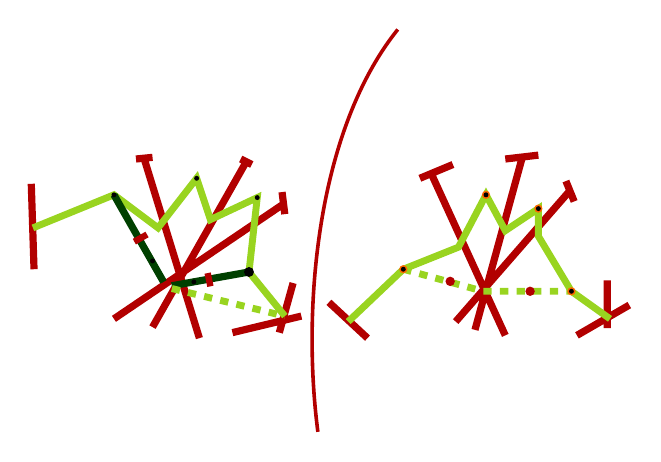
\begin{tikzpicture}[scale=.7]
\draw[red!70!black,line width=2.6pt] (0,2.8)--(.05,1.25) (2.05,3.25)--(3.05,0) (1.9,3.25)--(2.2,3.28) (2.2,.2)--(3.9,3.2) (3.8,3.25)--(4,3.15) (1.5,.35)--(4.6,2.45) (4.6,2.25)--(4.55,2.65) (3.65,.1)--(4.9,.4) (4.5,.1)--(4.75,1);
\draw[yellow!60!green,line width=2.5pt] (.03,2)--(1.5,2.6)--(2.3,2)--(3,2.9)--(3.25,2.15)--(4.1,2.55)--(3.95,1.2)--(4.6,.4);
\draw[green!25!black,line width=2.6pt] (1.5,2.6)--(2.4,1.02) (2.55,.95)--(3.95,1.2);
\draw[yellow!60!green,line width=2.5pt,dashed] (2.55,.9)--(4.6,.4);
\draw[red!70!black,line width=2.3pt] (1.87,1.75)--(2.1,1.88) (3.25,.94)--(3.2,1.18);
\foreach \p in {(1.5,2.6),(3,2.9),(4.1,2.55),(2.2,1.4),(2.95,1.02)}{\fill \p circle(.045);}
\fill (3.95,1.2) circle(.09);
\draw[red!70!black,line width=1.3pt] (6.65,5.6)..controls (5.2,3.8) and (4.9,.6)..(5.2,-1.7);
\begin{scope}[shift={(5.7,.2)}]
\draw[red!70!black,line width=2.6pt] (-.3,.45)--(.4,-.2) (1.55,2.8)--(2.9,-.15) (1.35,2.7)--(1.95,2.95) (2.35,-.05)--(3.2,3.05) (2.9,3.05)--(3.5,3.12) (2,.1)--(4.05,2.45) (4,2.65)--(4.15,2.28) (4.2,-.15)--(5.15,.4) (4.75,-.02)--(4.75,.85);
\draw[yellow!60!green,line width=2.5pt] (.05,.1)--(1.05,1.05)--(2.05,1.45)--(2.55,2.4)--(2.9,1.75)--(3.5,2.15)--(3.5,1.65)--(4.1,.65)--(4.8,.15);
\draw[yellow!60!green,line width=2.5pt,dashed] (1.05,1.05)--(2.5,.65)--(4.1,.65);
\foreach \p in {(1.05,1.05),(2.55,2.4),(3.5,2.15),(4.1,.65)}{\fill[orange!80!red] \p circle(.075); \fill \p circle(.045);}
\fill[red!70!black] (1.9,.83) circle(.085) (3.35,.65) circle(.085);
\end{scope}
\end{tikzpicture}}
\mspage{52}
\scanpage{54}
% E: text|upper left, instruction|Réécrit sans utiliser
\uline{\unsure{Réécrit|Récrit}} sans utiliser la position des arcs critiques, pour déterminer les signes de \(\varepsilon_{F'}(\deleted{\unsure{\alpha}}a')\), quand on connaît \deleted{\unsure{les signes}} \(\varepsilon_F(a)\).

\deleted{
% E: text|left upper, rejected proposition|Considérons l'ens V_F
\uline{Proposition}. Considérons l'ens \deleted{\unsure{de}} \(V_F\) (``\(\mathrm{vert}^4\)'') des sommets d'ordre 4 incidents à \(F\), et l'ens \(\sigma_a^{F'}(V_{F'})\) (où \(F'\) est la face incidente à \(F\) le long de le grand côté \(a\) de \(\delta F\)).

\deleted{Soit \unsure{\(\sigma_a(V_{F'})\)}} \unsure{les réunir dans décomposition} de \(\delta F\) en \deleted{\unsure{grands côtés}}\inserted{côtés} \unsure{considérés les} (fermés) \(\alpha\),
}

% E: text|left middle, new definition|Soit A_F a
Soit \(A_{F,a}=\unsure{A}\) la réunion des grands côtés en \(F\) qui sont telles que \(\sigma_a(\unsure{\alpha})\) est un grand côté de \(F'=\sigma_a(F)\) (NB \(a\) est un grand côté de \(F\)) Alors

% E: text|left lower, a|A est un arc
a) \(A\) est un arc sur \(\delta F\), soit \(B\) l'arc ``complémentaire''

\deleted{Alors} Considérons la subdivision de \(B\) en grands côtés (sommets verts clairs) et en ``grands côtés pour \(F'\)'' (sommets verts foncés). Alors le nb d'arêtes \(n_a(F)\) et \(n_a(F')\) qui interviennent est \unsure{compris} entre 3 et 5 --- les possibilités sont (\unsure{à un échange identique|à un échange} de \(F\) et \(F'\)) \(\unsure{(3,2)},\unsure{(3,3)},\unsure{(3,5)|(3,4)}\) \deleted{\unsure{Dans le cas particulier \(1)\ 2)\ 2)\)}} --- et dans tous les cas, c'est la face spéciale qui donne lieu à \unsure{3} arcs (ce qui suffit à le déterminer, quand on est dans le cas \(1^\circ\) ou \(3^\circ\)). De plus, on a

% E: text|right upper, b|Si alpha est une arête
b) Si \(\alpha\) est une\deleted{petite} arête de \(F\) dans \(A\), \deleted{\unsure{alors}} et \(\alpha\ne a\), on a \(\varepsilon_{F'}(\unsure{a|\alpha})=\varepsilon_F(\unsure{a|\alpha})\)

\([\mathrm{NB}\) si \(\alpha=a\), on a \(\varepsilon_{F'}(a)=-\varepsilon_F(a)]\)

% E: text|right upper-middle, c|On a les trois cas suivants
c) On a les \deleted{\unsure{pts}} trois cas suivants pour la distribution des grands côtés sur \(B\) (à échange près de \(F\) et \(F'\)) et les signes correspondants

% E: drawing|right middle, cancelled case 1|arch u x r y v epsilon signs
% E: drawing|right middle, cancelled case 2|arch u x r s y v
% E: drawing|right middle lower, cancelled empty arch|1 degree green arch
\deleted{\figure{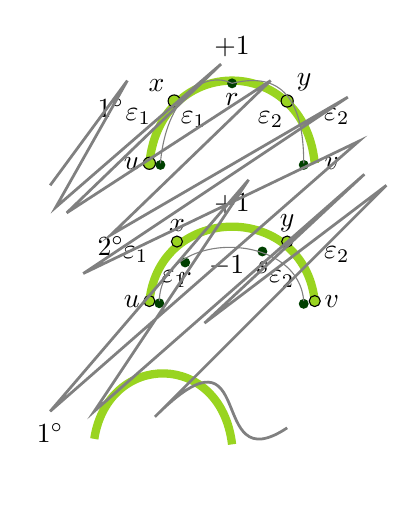
\begin{tikzpicture}[scale=.7]
\node at (-.7,1) {$1^\circ$};
\draw[yellow!60!green,line width=3pt] (0,0)..controls (.2,2) and (2.8,2)..(3,0);
\foreach \p in {(0,0),(.45,1.13),(2.5,1.13)}{\fill[yellow!60!green] \p circle(.11); \draw \p circle(.11);}
\fill[green!25!black] (1.5,1.45) circle(.09) (.2,-.03) circle(.09) (2.8,-.03) circle(.09);
\node[left] at (0,0) {$u$}; \node[above left] at (.45,1.13) {$x$}; \node[above right] at (2.5,1.13) {$y$}; \node[right] at (3,0) {$v$};
\node[below] at (1.5,1.45) {$r$}; \node[above] at (1.5,1.75) {$+1$};
\draw[gray] (.2,0)..controls (.3,1.2) and (1,1.7)..(1.5,1.45)..controls (2.5,1.7) and (2.8,1)..(2.8,0);
\node at (.8,.8) {$\varepsilon_1$}; \node at (2.2,.8) {$\varepsilon_2$}; \node at (-.2,.85) {$\varepsilon_1$}; \node at (3.4,.85) {$\varepsilon_2$};
\begin{scope}[shift={(0,-2.5)}]
\node at (-.7,1) {$2^\circ$};
\draw[yellow!60!green,line width=3pt] (0,0)..controls (.2,1.8) and (2.8,1.8)..(3,0);
\foreach \p in {(0,0),(.5,1.08),(2.5,1.08),(3,0)}{\fill[yellow!60!green] \p circle(.1); \draw \p circle(.1);}
\foreach \p in {(.18,-.04),(.65,.7),(2.05,.9),(2.8,-.05)}{\fill[green!25!black] \p circle(.09);}
\node[left] at (0,0) {$u$}; \node[above] at (.5,1.08) {$x$}; \node[above] at (2.5,1.08) {$y$}; \node[right] at (3,0) {$v$}; \node[below] at (.65,.7) {$r$}; \node[below] at (2.05,.9) {$s$};
\node at (1.4,.65) {$-1$}; \node[above] at (1.5,1.4) {$+1$};
\draw[gray] (.18,0)..controls (.2,1.3) and (2.7,1.3)..(2.8,0);
\node at (.45,.4) {$\varepsilon_1$}; \node at (2.4,.4) {$\varepsilon_2$}; \node at (-.25,.85) {$\varepsilon_1$}; \node at (3.4,.85) {$\varepsilon_2$};
\end{scope}
\node at (-1.8,-4.9) {$1^\circ$};
\draw[yellow!60!green,line width=3pt] (-1,-5)..controls (-.75,-3.4) and (1.3,-3.4)..(1.5,-5.1);
\draw[gray,line width=1pt] (-1.8,-.4)--(-.4,1.5)--(-1.7,-.8)--(1.3,1.8)--(-1.5,-.9)--(2.2,1.5)--(-.7,-1.3)--(3.6,1.2)--(-1.2,-2)--(3.8,.4)--(-1.8,-4.5)--(1.8,-.3)--(-1,-4.5)--(3.9,-.2)--(1,-2.9)--(4.3,-.4)--(.1,-4.6)..controls (2,-2.7) and (1,-5.8)..(2.5,-4.8);
\end{tikzpicture}}}

% E: drawing|right lower-middle, revised case 1|u x r y v arch signs epsilon1 epsilon2
\figure{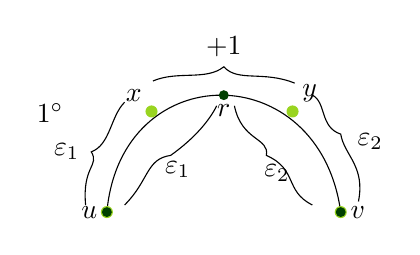
\begin{tikzpicture}[scale=.9]
\node at (-.8,1.4) {$1^\circ$};
\draw (0,0)..controls (.2,2.2) and (3,2.2)..(3.3,0);
\foreach \p in {(0,0),(.63,1.42),(2.62,1.42),(3.3,0)}{\fill[yellow!60!green] \p circle(.085);}
\foreach \p in {(0,0),(1.65,1.65),(3.3,0)}{\fill[green!25!black] \p circle(.07);}
\node[left] at (0,0) {$u$}; \node[above left] at (.63,1.42) {$x$}; \node[above right] at (2.62,1.42) {$y$}; \node[right] at (3.3,0) {$v$}; \node[below] at (1.65,1.65) {$r$};
\draw (.65,1.85)..controls (1,2) and (1.4,1.85)..(1.65,2.05)..controls (1.85,1.83) and (2.2,2)..(2.65,1.82);
\node[above] at (1.65,2.05) {$+1$};
\draw (-.3,.1)..controls (-.35,.65) and (-.1,.65)..(-.22,.85)..controls (.05,.95) and (.05,1.35)..(.25,1.55);
\node[left] at (-.25,.85) {$\varepsilon_1$};
\draw (2.9,1.65)..controls (3.1,1.55) and (3,1.2)..(3.3,1.1)..controls (3.35,.8) and (3.65,.65)..(3.55,.15);
\node[right] at (3.4,1) {$\varepsilon_2$};
\draw (.25,.1)..controls (.6,.45) and (.55,.75)..(.9,.8)..controls (1.25,1.05) and (1.45,1.3)..(1.55,1.5);
\node at (1,.6) {$\varepsilon_1$};
\draw (1.8,1.5)..controls (1.9,1) and (2.3,1.05)..(2.25,.8)..controls (2.7,.6) and (2.5,.3)..(2.9,.1);
\node at (2.4,.55) {$\varepsilon_2$};
\end{tikzpicture}}

% E: drawing|right lower, revised case 2|u r x s y v plus one minus one
\figure{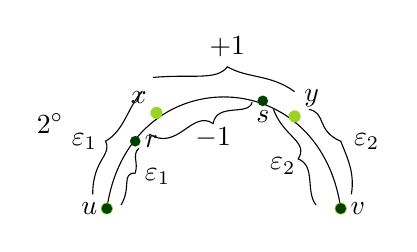
\begin{tikzpicture}[scale=.9]
\node at (-.8,1.2) {$2^\circ$};
\draw (0,0)..controls (.3,2.1) and (3,2.1)..(3.3,0);
\foreach \p in {(0,0),(.7,1.35),(2.65,1.3),(3.3,0)}{\fill[yellow!60!green] \p circle(.085);}
\foreach \p in {(0,0),(.4,.95),(2.2,1.52),(3.3,0)}{\fill[green!25!black] \p circle(.075);}
\node[left] at (0,0) {$u$}; \node[above left] at (.7,1.35) {$x$}; \node[above right] at (2.65,1.3) {$y$}; \node[right] at (3.3,0) {$v$}; \node[right] at (.4,.95) {$r$}; \node[below] at (2.2,1.52) {$s$};
\draw (.65,1.85)..controls (1.2,1.9) and (1.55,1.8)..(1.7,2)..controls (2,1.83) and (2.3,1.9)..(2.65,1.65);
\node[above] at (1.7,2) {$+1$};
\draw (.6,1.05)..controls (1,.8) and (1.2,1.4)..(1.5,1.2)..controls (1.55,1.5) and (2,1.3)..(2.05,1.5);
\node at (1.5,1) {$-1$};
\draw (-.2,.2)..controls (-.2,.7) and (.08,.75)..(-.02,.95)..controls (.25,1.1) and (.3,1.45)..(.5,1.65);
\node[left] at (0,.95) {$\varepsilon_1$};
\draw (.2,.05)..controls (.35,.3) and (.2,.5)..(.4,.5)..controls (.45,.65) and (.35,.75)..(.45,.85);
\node[right] at (.4,.45) {$\varepsilon_1$};
\draw (2.35,1.4)..controls (2.5,1) and (2.85,.95)..(2.7,.7)..controls (2.95,.6) and (2.8,.25)..(2.95,.05);
\node[left] at (2.8,.6) {$\varepsilon_2$};
\draw (2.85,1.4)..controls (3.1,1.35) and (2.95,1.1)..(3.3,.95)..controls (3.4,.7) and (3.5,.5)..(3.45,.2);
\node[right] at (3.35,.95) {$\varepsilon_2$};
\end{tikzpicture}}

% E: drawing|bottom right, revised case 3|arch with three dark interior vertices
\figure{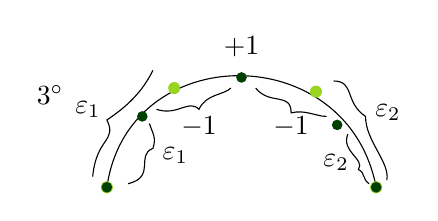
\begin{tikzpicture}[scale=.9]
\node at (-.8,1.3) {$3^\circ$};
\draw (0,0)..controls (.3,2.1) and (3.4,2.1)..(3.8,0);
\foreach \p in {(0,0),(.95,1.4),(2.95,1.35),(3.8,0)}{\fill[yellow!60!green] \p circle(.085);}
\foreach \p in {(0,0),(.5,1),(1.9,1.55),(3.25,.88),(3.8,0)}{\fill[green!25!black] \p circle(.075);}
\node[above] at (1.9,1.7) {$+1$};
\draw (.7,1.1)..controls (1,1) and (1.15,1.25)..(1.3,1.1)..controls (1.4,1.32) and (1.65,1.3)..(1.75,1.4);
\draw (2.1,1.4)..controls (2.3,1.15) and (2.6,1.35)..(2.6,1.05)..controls (2.8,1.1) and (2.95,1)..(3.1,1);
\node at (1.3,.85) {$-1$}; \node at (2.6,.85) {$-1$};
\draw (-.2,.15)..controls (-.15,.7) and (.15,.65)..(0,.95)..controls (.3,1.15) and (.5,1.35)..(.65,1.65);
\node[left] at (.05,1.1) {$\varepsilon_1$};
\draw (.3,.05)..controls (.7,.15) and (.4,.45)..(.65,.55)..controls (.7,.7) and (.65,.75)..(.6,.9);
\node[right] at (.65,.45) {$\varepsilon_1$};
\draw (3.4,.75)..controls (3.3,.5) and (3.65,.4)..(3.55,.25)..controls (3.65,.2) and (3.6,.12)..(3.7,.05);
\node[left] at (3.55,.35) {$\varepsilon_2$};
\draw (3.2,1.5)..controls (3.5,1.5) and (3.35,1.2)..(3.65,1)..controls (3.65,.65) and (4,.35)..(3.95,.1);
\node[right] at (3.65,1.05) {$\varepsilon_2$};
\end{tikzpicture}}
\mspage{53}
\scanpage{55}
% E: text|left upper, corollary|Dans tous les cas
\uline{Corollaire} Dans tous les cas, la distribution des signes \(\varepsilon_{\unsure{a|\cdot}}(F)\) détermine celle des \(\varepsilon_{\unsure{a'|\cdot}}(F')\). \deleted{C'est clair \unsure{et}}

% E: text|left upper-middle, proof|C'est clair d'abord
C'est clair d'abord dans les cas \(1^\circ\) et \(3^\circ\), où on sait laquelle des faces \(F,F'\) est la spécialisée de l'autre ; \deleted{et par suite}\inserted{Mais} dans le cas\inserted{``symétrique''} \((2^\circ)\), \deleted{\unsure{comme on connaît les signes \(\varepsilon(F)\), on}} On voit que \deleted{les} deux\inserted{grands} côtés extérieurs correspondants pour \(F,F'\) ont $=$ \uline{signe} (c'est tjrs le cas, y compris dans les cas \(1^\circ\) et \(2^\circ\)), et pour les côtés qui \unsure{restent}\inserted{\unsure{en}} par dessus, elles sont (pour \(F,F'\) \unsure{par \(\sigma\)}) toutes de $=$ signe (\uline{NB} leur nb, suivant les cas, est \((1,0),(1,1)\) ou \((1,2)\)) et les signes en question pour \(F\) et pour \(F'\) sont opposés.

% E: text|left bottom, second corollary|Quand on connaît les signes
\uline{Corollaire} Quand on connaît les signes \(\varepsilon_F(\unsure{a})\) pour \uline{une} face \(F\), on les connaît pour \uline{tous} (grâce à la connexité de \(X\))

% E: text|right upper, qualification|J'ai supposé implicitement
J'ai supposé implicitement \deleted{que} dans la vérification de la proposition que ni \(F\), ni \(F'\) n'est une face exceptionnelle (i.e. ne correspondant à une position \unsure{ultime|critique} exceptionnelle, i.e. ``supercritique''). Il faudrait que j'examine séparément le cas de telles faces.

% E: text|right middle, exceptional face|Pour une telle face
Pour une telle face, il n'y a \unsure{que|pas} quatre grands côtés, et la distribution des signes est connue --- Cela semble donner une façon simple de déduire les signes\inserted{ou les rôles} de la seule structure de carte de \((X,K,S_K)\), sans avoir à utiliser les arcs critiques, et encore moins \deleted{les} le \deleted{\unsure{complexe}} graphe \(L\subset X\).
\mspage{54}
\scanpage{56}
% E: display|upper left, pencil sum|nu_s1 minus one
\[
(\nu_{s_1}-1)+(\nu_{s_2}-1)\unsure{\cdots|+\cdots}
 +(\nu_{\unsure{s_n|s_0}}-1)
\]
\inserted{\(\unsure{\nu_{s_0}}\)}

% E: drawing|upper left|circle with three attached polygons arrows zero one
\figure{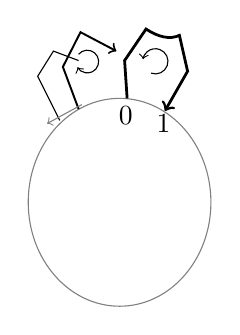
\begin{tikzpicture}[scale=.8]
\draw[gray] (0,0) ellipse(1.45 and 1.65);
\draw (-.95,1.3)--(-1.3,2)--(-1.05,2.4)--(-.65,2.25);
\draw[line width=.7pt,->] (-.65,1.48)--(-.9,2.15)--(-.62,2.7)--(-.05,2.4);
\draw[line width=1pt,->] (.12,1.65)--(.08,2.25)--(.42,2.75)..controls (.62,2.62) and (.8,2.58)..(.95,2.65)--(1.08,2.08)--(.72,1.45);
\draw[->] (-.65,2.35) arc(140:-150:.18); \draw[->] (.5,2.05) arc(-110:170:.2);
\draw[gray,->] (-.6,1.55)--(-1.15,1.25);
\node at (.1,1.37) {$0$}; \node at (.7,1.25) {$1$};
\end{tikzpicture}}

% E: drawing|upper centre-left|vertical interval with s1 s0 s n-1
\figure{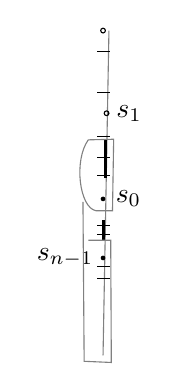
\begin{tikzpicture}[scale=.75]
\draw[gray] (0,0)--(.1,5.5);
\draw (0,5.5) circle(.04) (.06,4.1) circle(.04);
\foreach \y in {1.3,1.5,2.05,2.2,3.05,3.35,3.7,4.45,5.15}{\draw (-.1,\y)--(.12,\y);}
\fill (0,2.65) circle(.04) (0,1.65) circle(.04);
\node[right] at (.06,4.1) {$s_1$}; \node[right] at (.05,2.65) {$s_0$}; \node[left] at (0,1.65) {$s_{n-1}$};
\draw[line width=1.1pt] (.04,3)--(.04,3.65) (0,1.95)--(0,2.3);
\draw[gray] (-.25,3.65)..controls (-.5,3.3) and (-.4,2.5)..(-.12,2.45)--(.16,2.45)--(.18,3.66)--cycle;
\draw[gray] (-.34,2.6)--(-.32,-.1)--(.14,-.12)--(.13,1.95)--(-.25,1.95);
\end{tikzpicture}}

% E: display|left middle, lengths|l_s equals n minus nu_s
\[
\begin{aligned}
\ell_s&=\deleted{\unsure{\ell_0}}n-\nu_s\\
\ell_a&=\deleted{\unsure{\ell}}n-1-(\nu_s-1)-(\nu_t-1)\\
&=n\deleted{\unsure{+}}\inserted{-}(\nu_s+\nu_t-1)=(n-\nu_s)-(\nu_t-1)\\
\ell_s-\ell_a&=\nu_t-1\qquad \unsure{=|\geq}\deleted{\unsure{\nu_t}}\unsure{1}
\end{aligned}
\]

% E: display|left middle-lower, sum|chi_2n sum multiplicities
\[
\chi_{2n}(\unsure{s|0})=\sum_{\substack{s\ \text{\unsure{tournant}}\\\text{sur }D_i}}(\nu(s)-1)=n-1
\qquad \mathbb Z/N\mathbb Z
\]
\inserted{multiplicité des sommets}

% E: display|left lower, lambda|lambda equals rho tilde
\[
\lambda(t)=\widetilde{\rho}_p(t)=(-1)^p(t-\chi_p)
\]
% E: text|left lower, parity|ici p equals 2n
ici \(p=2n\) donc \((-1)^p=+1\)

\deleted{\unsure{\(\rho\)}}\deleted{\(t\mapsto\)}
% E: display|left lower, simplified lambda|t minus chi_2n
\[
\lambda(t)=\deleted{\unsure{\ell}}t-\chi_{2n}=t-(n-1)
\]

% E: text|left bottom, NB|rho_p composition
\uline{NB}
\[
\begin{aligned}
\rho_p(t)&=\sigma_{p-1}\cdots\sigma_0(t)
=\deleted{(-1)^{p-1}(\chi_{\unsure{p|p-1}}-t)}\inserted{(-1)^p(t-\chi_p)}\\
&\deleted{=(-1)^p t+(-1)^{p-1}\chi_p}
\end{aligned}
\]

% E: text|bottom left, passage|Passage de F_p a F_0
Passage de \(F_p\) à \(F_0\) se fait par \(t\mapsto\deleted{\unsure{\ell_p-t}}t\)
\deleted{\unsure{(en effet, \(\ell_0=0\))}}

% E: drawing|central vertical face sequence|F p-1 F p F0 F1 F2 Fn Fn+1
\figure{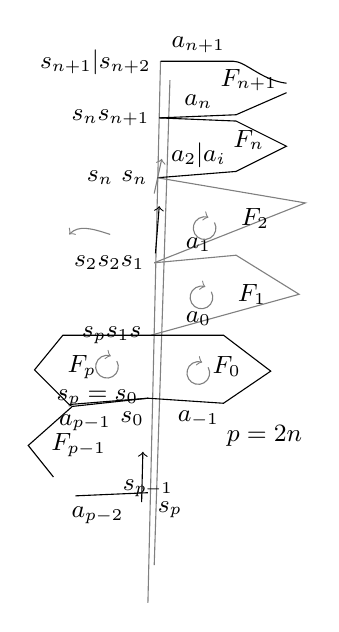
\begin{tikzpicture}[x=.8cm,y=.8cm,font=\small]
\draw[gray] (0,-1.4)--(.2,7.2);
\draw[gray] (.1,-.8)--(.35,6.9);
\draw[->] (-.1,.2)--(-.08,1); \draw[->] (.12,4.15)--(.18,4.9);
\draw[gray,->] (.1,5.1)--(.22,5.65);
\draw (.2,7.2)--(1.35,7.2)..controls (1.55,7.2) and (1.8,6.9)..(2.2,6.85);
\draw (2.2,6.7)--(1.4,6.35)--(.18,6.3);
\draw (.18,6.3)--(1.4,6.25)--(2.2,5.85)--(1.4,5.45)--(.15,5.35);
\draw[gray] (.15,5.35)--(2.5,4.95)--(.1,4);
\draw[gray] (.1,4)--(1.4,4.12)--(2.4,3.5)--(.05,2.85);
\draw (.05,2.85)--(1.2,2.85)--(1.95,2.28)--(1.2,1.77)--(0,1.85);
\draw (0,1.85)--(-1.25,1.75)--(-1.8,2.3)--(-1.35,2.85)--(.05,2.85);
\draw (0,1.85)--(-1.2,1.72)--(-1.9,1.1)--(-1.5,.6) (-1.15,.3)--(0,.35);
\node at (1.6,6.9) {$F_{n+1}$}; \node at (1.6,5.95) {$F_n$}; \node at (1.7,4.7) {$F_2$}; \node at (1.65,3.5) {$F_1$}; \node at (1.25,2.35) {$F_0$};
\node at (-1.05,2.35) {$F_p$}; \node at (-1.1,1.1) {$F_{p-1}$};
\node[above] at (.8,7.18) {$a_{n+1}$}; \node[left] at (.2,7.18) {$\unsure{s_{n+1}|s_{n+2}}$};
\node[above] at (.8,6.3) {$a_n$}; \node[left] at (.18,6.3) {$\deleted{\unsure{s_n}}s_{n+1}$};
\node[above] at (.8,5.35) {$\unsure{a_2|a_i}$}; \node[left] at (.15,5.35) {$s_n\ \unsure{s_n}$};
\node[above] at (.8,4.02) {$a_1$}; \node[left] at (.1,4) {$\deleted{\unsure{s_2}}s_2\unsure{s_1}$};
\node[above] at (.8,2.85) {$a_0$}; \node[left] at (.05,2.85) {$\unsure{s_p}\deleted{\unsure{s_1}}s$};
\node[below] at (.8,1.8) {$a_{-1}$}; \node[left] at (0,1.85) {$s_p=s_0$};
\node at (-.25,1.52) {$\deleted{\unsure{s_0}}$};
\node[below] at (-1,1.75) {$a_{p-1}$}; \node[below] at (-.8,.28) {$a_{p-2}$};
\node at (0,.42) {$\unsure{s_{p-1}}$}; \node at (.35,.08) {$\deleted{\unsure{s_p}}$};
\node at (1.85,1.25) {$p=2n$};
\foreach \xx/\yy in {.8/2.25,.85/3.45,.9/4.55,-.65/2.35}{\draw[gray,->] (\xx,\yy) ++(30:.18) arc(30:-290:.18);}
\draw[gray,->] (-.6,4.45)..controls (-.9,4.55) and (-1.1,4.6)..(-1.25,4.45);
\end{tikzpicture}}

% E: drawing|lower centre, pencil circle|circle surrounded by curved petals
\figure{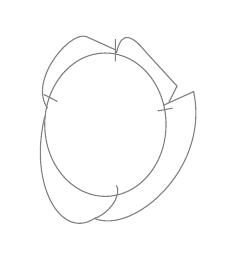
\begin{tikzpicture}[scale=.7]
\draw[gray] (0,0) ellipse (1.1 and 1.3);
\draw[gray] (-1.05,.3)..controls (-1.4,.8) and (-.65,1.7)..(-.35,1.6)--(.2,1.35);
\draw[gray] (.2,1.3)..controls (.3,1.75) and (.5,1.6)..(.75,1.3)--(1.3,.7)--(1.15,.4);
\draw[gray] (1.05,.35)--(1.6,.6)..controls (1.9,-.8) and (.5,-2)..(-.2,-1.7);
\draw[gray] (-1.1,.15)..controls (-1.4,-1.1) and (-.8,-2.1)..(-.2,-1.7)..controls (.1,-1.6) and (.3,-1.25)..(.2,-1.1);
\draw[gray] (-1.12,.55)--(-.87,.42) (.95,.25)--(1.22,.3) (.18,1.55)--(.18,1.15);
\end{tikzpicture}}

% E: diagram|right upper, element mapping|s n+1 maps to s n+1
\diagram{\begin{tikzcd}
s_{n+1}\arrow[r,mapsto] & s_{n+1}
\end{tikzcd}}

% E: diagram|right upper, square|P Fn to P Fn+1 and Z NZ
\diagram{\begin{tikzcd}
\unsure{P(F_n)|\operatorname{Pol}(F_n)}\arrow[r,"\sigma_{a_n}"] & \unsure{P(F_{n+1})|\operatorname{Pol}(F_{n+1})}\\
\mathbb Z/N\mathbb Z\arrow[u,no head,"\varphi_n","\wr"']\arrow[r,"\sigma_n"] & \deleted{\unsure{P}}\mathbb Z/N\mathbb Z\arrow[u,no head,"\varphi_{n+1}"',"\wr"]
\end{tikzcd}}

% E: text|right middle, properties|sigma_n respecte
\(\sigma_n\) respecte la structure polygonale

b) renverse l'orientation

c) transforme \(\underbrace{\varphi_n^{-1}(s_{n+1})}_{\ell_n}\) en \(\underbrace{\varphi_{n+1}^{-1}(s_{n+1})}_{0}\)

% E: display|right middle, conclusion|sigma_n t equals l_n minus t
donc \(\sigma_n(t)=\ell_n-t\)

% E: display|lower centre, three individual maps|sigma zero one n
\[
\begin{aligned}
\sigma_0(t)&=\ell_0-t\\
\sigma_1(t)&=\ell_1-t\\
\sigma_n(t)&=\ell_n-t
\end{aligned}
\]

% E: display|right lower, compositions|sigma1 sigma0
\[
\begin{aligned}
\sigma_1\sigma_0(t)&=\ell_1-(\ell_0-t)=\ell_1-\ell_0+t\\
\sigma_2\sigma_1\sigma_0(t)&=\ell_2-\ell_1+\ell_0-t\\
\underbrace{\overbrace{(\sigma_n\deleted{\unsure{\sigma}}\sigma_{n-1}\cdots\sigma_0)}^{n+1\ \text{facteurs}}}_{\rho_{n+1}}(t)
&=\ell_n-\ell_{n-1}\unsure{-\cdots|+\cdots}+(-1)^n\ell_0+(-1)^{n+1}t\\
&=(-1)^n(\chi_{n+1}-t)=(-1)^{n+1}(t-\chi_{n+1})
\end{aligned}
\]
% E: display|right bottom, alternating sum|chi n+1
où \(\displaystyle\chi_{n+1}=\underbrace{\ell_0\unsure{-|+}\ell_1\cdots+(-1)^n\ell_n}_{n+1\ \text{termes}}\)

% E: display|bottom edge, unfinished formula|sigma p-1 sigma p
\[
\underbrace{\sigma_{p-1}\sigma_{\unsure{p|p-2}}\cdots\sigma_0}_{\unsure{\rho_p}}(t)=(-1)^{p-1}
\]
\mspage{55}
\scanpage{57}
% E: text|printed header upper left|//* CRAY2 0296 I
\texttt{//*\quad CRAY2\quad 0296\qquad I}
% E: display|top handwritten calculation|nu(n-1)+nu(n-3)
\[
\nu(\underbrace{n-1}_{\unsure{2}})+\nu(n-3)=2\nu n-4\nu
\deleted{{}=2\nu(n-1)}\qquad\deleted{{}=\nu(2n-3)}
\]
\[=\boxed{2\nu(n-2)}\]
\[\unsure{2(n-2)}\]
% E: drawing|top right at torn corner|pentagon labelled 0 1 2 3 4
\figure{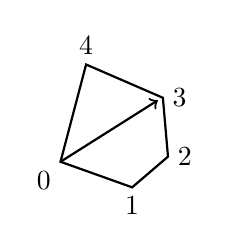
\begin{tikzpicture}[scale=.65]
\draw[thick] (0,0)--(1.4,-.5)--(2.1,.1)--(2,1.25)--(.5,1.9)--cycle;
\draw[->,thick] (0,0)--(1.9,1.2);
\node[below left] at (0,0) {$0$};\node[below] at (1.4,-.5) {$1$};\node[right] at (2.1,.1) {$2$};\node[right] at (2,1.25) {$3$};\node[above] at (.5,1.9) {$\unsure{4}$};
\end{tikzpicture}}
% E: drawing|printed upper banner|0051 formed from repeated digits
\figure{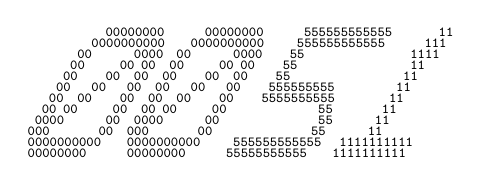
\begin{tikzpicture}[x=.09cm,y=.14cm,every node/.style={font=\tiny\ttfamily,anchor=west,inner sep=0pt}]
\foreach \d in {0,14}{
\node at ({\d+11},0) {00000000};\node at ({\d+9},-1) {0000000000};
\node at ({\d+7},-2) {00};\node at ({\d+15},-2) {0000};
\node at ({\d+6},-3) {00};\node at ({\d+13},-3) {00};\node at ({\d+16},-3) {00};
\node at ({\d+5},-4) {00};\node at ({\d+11},-4) {00};\node at ({\d+15},-4) {00};
\node at ({\d+4},-5) {00};\node at ({\d+9},-5) {00};\node at ({\d+14},-5) {00};
\node at ({\d+3},-6) {00};\node at ({\d+7},-6) {00};\node at ({\d+13},-6) {00};
\node at ({\d+2},-7) {00};\node at ({\d+5},-7) {00};\node at ({\d+12},-7) {00};
\node at ({\d+1},-8) {0000};\node at ({\d+11},-8) {00};
\node at (\d,-9) {000};\node at ({\d+10},-9) {00};
\node at (\d,-10) {0000000000};\node at (\d,-11) {00000000};}
\node at (39,0) {555555555555};\node at (38,-1) {555555555555};
\node at (37,-2) {55};\node at (36,-3) {55};\node at (35,-4) {55};
\node at (34,-5) {555555555};\node at (33,-6) {5555555555};
\node at (41,-7) {55};\node at (41,-8) {55};\node at (40,-9) {55};
\node at (29,-10) {555555555555};\node at (28,-11) {55555555555};
\node at (58,0) {11};\node at (56,-1) {111};\node at (54,-2) {1111};
\foreach \r in {3,4,5,6,7,8,9}{\node at ({57-\r},-\r) {11};}
\node at (44,-10) {1111111111};\node at (43,-11) {1111111111};
\end{tikzpicture}}
% E: drawing|upper left over the printed digits|narrow brown loops and strokes
\figure{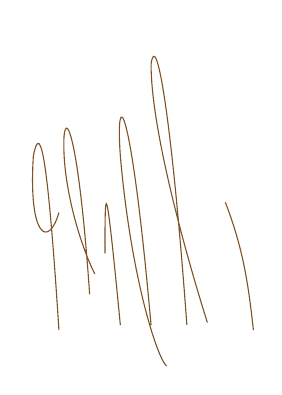
\begin{tikzpicture}[scale=.65]
\draw[brown!65!black,thin] (0,0)..controls (-.2,3.1) and (-.35,4.2)..(-.5,3.4)..controls (-.6,1.8) and (-.2,1.6)..(0,2.3)
(.6,.7)..controls (.4,3.6) and (.15,4.3)..(.1,3.8)..controls (.05,2.9) and (.4,1.7)..(.7,1.1)
(1.2,.1)..controls (.9,3.2) and (.9,2.8)..(.9,1.5)
(1.8,.1)..controls (1.4,4.6) and (1.1,4.8)..(1.2,3.4)..controls (1.4,1.1) and (1.9,-.5)..(2.1,-.7)
(2.5,.1)..controls (2.2,4.2) and (1.9,5.9)..(1.8,5.2)..controls (1.8,3.8) and (2.6,1.1)..(2.9,.15)
(3.8,0)..controls (3.7,.9) and (3.6,1.6)..(3.25,2.5);
\end{tikzpicture}}
% E: drawing|upper row left green polygon|inverted (3,5)
% E: drawing|upper row middle green polygon|inverted (3,4)
% E: drawing|upper row right green polygon|inverted (3,3)
% E: drawing|upper row separating line|vertical green line
\figure{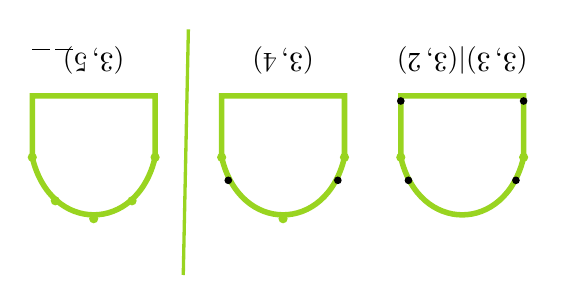
\begin{tikzpicture}[scale=.65]
\foreach \d in {0,3.7,7.2}{\draw[yellow!60!green,line width=2pt] (\d,2)--({\d+2.4},2)--({\d+2.4},.8)..controls ({\d+2.05},-.7) and ({\d+.35},-.7)..(\d,.8)--cycle;
\foreach \x/\y in {0/.8,2.4/.8}{\fill[yellow!60!green] ({\d+\x},\y) circle(.09);}}
\foreach \p in {(.45,-.05),(1.2,-.4),(1.95,-.05),(4.9,-.4)}{\fill[yellow!60!green] \p circle(.09);}
\foreach \p in {(3.83,.35),(5.97,.35),(7.2,1.9),(9.6,1.9),(7.35,.35),(9.45,.35)}{\fill \p circle(.075);}
\node[rotate=180] at (1.2,2.7) {$\unsure{(3,5)}$};\node[rotate=180] at (4.9,2.7) {$(3,4)$};\node[rotate=180] at (8.4,2.7) {$\unsure{(3,3)|(3,2)}$};
\draw[yellow!60!green,line width=1.2pt] (3.05,3.3)--(2.95,-1.5);
\draw (0,2.9)--(.35,2.9) (.45,2.9)--(.8,2.9);
\end{tikzpicture}}
% E: drawing|upper right below pentagon|diamond with arrow and numbered vertices
% E: drawing|upper right beside diamond|trapezoid thick lower edge
% E: drawing|right centre pencil oval|oval with lower label 1
\figure{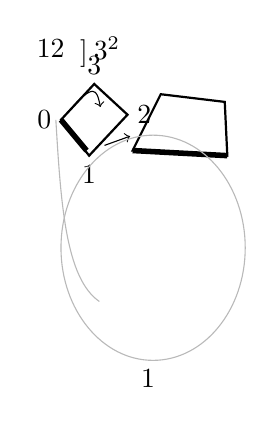
\begin{tikzpicture}[scale=.65]
\node at (-.2,2.1) {$\unsure{12}$};\node at (.45,2) {$\unsure{]}$};\node at (.9,2.1) {$\unsure{3^{2}}$};
\draw[thick] (0,.7)--(.65,1.4)--(1.3,.8)--(.55,0)--cycle;
\draw[line width=2pt] (0,.7)--(.5,.1);\draw[->] (.12,.83)..controls (.65,1.45) and (.7,1.3)..(.77,.95);
\draw[->] (.85,.2)--(1.35,.38);
\node[left] at (0,.7) {$0$};\node[below] at (.55,0) {$1$};\node[right] at (1.3,.8) {$2$};\node[above] at (.65,1.4) {$3$};
\draw[thick] (1.4,.1)--(1.95,1.2)--(3.2,1.05)--(3.25,0)--cycle;
\draw[line width=2pt] (1.4,.1)--(3.25,0);
\draw[gray!55] (1.8,-1.8) ellipse (1.8 and 2.2);
\draw[gray!55] (-.1,.7)..controls (.0,-1) and (.1,-2.4)..(.75,-2.85);
\node[below] at (1.7,-4) {$\unsure{1}$};
\end{tikzpicture}}
% E: drawing|middle left pair of green polygons|inverted (3,3) (3,4) and minus-one braces
\figure{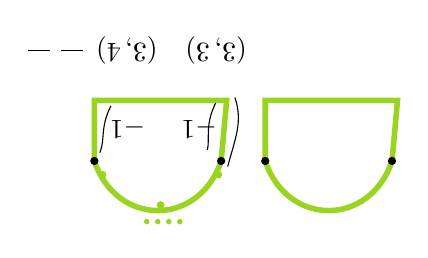
\begin{tikzpicture}[scale=.7]
\foreach \d in {0,3.1}{\draw[yellow!60!green,line width=2pt] (\d,2)--({\d+2.4},2)--({\d+2.3},.9)..controls ({\d+1.9},-.3) and ({\d+.4},-.3)..(\d,.9)--cycle;
\fill (\d,.9) circle(.075);\fill ({\d+2.3},.9) circle(.075);}
\foreach \p in {(.15,.65),(1.2,.1),(2.25,.65)}{\fill[yellow!60!green] \p circle(.07);}
\foreach \x in {.95,1.15,1.35,1.55}{\fill[yellow!60!green] (\x,-.2) circle(.05);}
\draw (2.55,2.05)..controls (2.7,1.6) and (2.55,1.3)..(2.42,.8);
\node[rotate=180] at (1.4,2.9) {$(3,3)\quad(3,4)$};
\node[rotate=180] at (.6,1.5) {$-1$};\node[rotate=180] at (1.9,1.5) {$-1$};
\draw (.3,1.9)..controls (.1,1.5) and (.2,1.3)..(.1,1.05) (2.2,1.95)..controls (2,1.55) and (2.1,1.3)..(2.05,1.1);
\draw (-.6,2.9)--(-.2,2.9) (-1.2,2.9)--(-.8,2.9);
\end{tikzpicture}}
% E: drawing|printed middle banner|CRAY2 formed from repeated characters
\figure{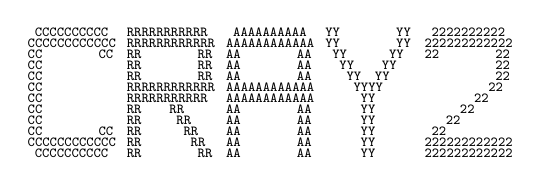
\begin{tikzpicture}[x=.09cm,y=.14cm,every node/.style={font=\tiny\ttfamily,anchor=west,inner sep=0pt}]
\node at (1,0) {CCCCCCCCCC}; \node at (0,-1) {CCCCCCCCCCCC};
\foreach \r in {2,3,4,5,6,7,8,9}{\node at (0,-\r) {CC};}
\node at (10,-2) {CC}; \node at (10,-9) {CC};
\node at (0,-10) {CCCCCCCCCCCC}; \node at (1,-11) {CCCCCCCCCC};
\node at (14,0) {RRRRRRRRRRR}; \node at (14,-1) {RRRRRRRRRRRR};
\foreach \r in {2,3,4,7,8,9,10,11}{\node at (14,-\r) {RR};}
\foreach \r in {2,3,4}{\node at (24,-\r) {RR};}
\node at (14,-5) {RRRRRRRRRRRR}; \node at (14,-6) {RRRRRRRRRRR};
\node at (20,-7) {RR}; \node at (21,-8) {RR}; \node at (22,-9) {RR}; \node at (23,-10) {RR}; \node at (24,-11) {RR};
\node at (29,0) {AAAAAAAAAA}; \node at (28,-1) {AAAAAAAAAAAA};
\foreach \r in {2,3,4,7,8,9,10,11}{\node at (28,-\r) {AA}; \node at (38,-\r) {AA};}
\node at (28,-5) {AAAAAAAAAAAA}; \node at (28,-6) {AAAAAAAAAAAA};
\foreach \r in {0,1}{\node at (42,-\r) {YY}; \node at (52,-\r) {YY};}
\node at (43,-2) {YY}; \node at (51,-2) {YY};
\node at (44,-3) {YY}; \node at (50,-3) {YY};
\node at (45,-4) {YY}; \node at (49,-4) {YY};
\node at (46,-5) {YYYY};
\foreach \r in {6,7,8,9,10,11}{\node at (47,-\r) {YY};}
\node at (57,0) {2222222222}; \node at (56,-1) {222222222222};
\node at (56,-2) {22}; \node at (66,-2) {22};
\node at (66,-3) {22}; \node at (66,-4) {22}; \node at (65,-5) {22}; \node at (63,-6) {22}; \node at (61,-7) {22}; \node at (59,-8) {22}; \node at (57,-9) {22};
\node at (56,-10) {222222222222}; \node at (56,-11) {222222222222};
\end{tikzpicture}}
% E: drawing|centre over listing|green circle with black arcs and red ticks
\figure{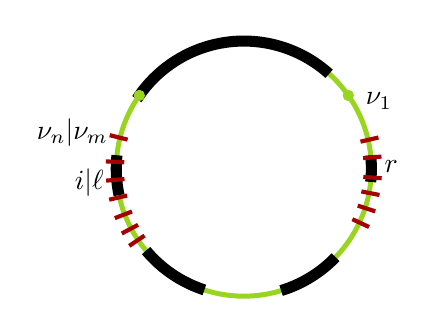
\begin{tikzpicture}[scale=.9]
\draw[yellow!60!green,line width=1.8pt] (0,0) circle(1.8);
\foreach \a/\b in {48/147,174/192,220/252,287/316,354/366}{\draw[line width=4pt] (\a:1.8) arc (\a:\b:1.8);}
\foreach \a in {145,35}{\fill[yellow!60!green] (\a:1.8) circle(.08);}
\foreach \a in {166,177,185,193,201,208,214,335,342,349,356,365,373}{\draw[red!65!black,line width=1.5pt] (\a:1.69)--(\a:1.95);}
\node[left] at (164:1.85) {$\unsure{\nu_n|\nu_m}$};\node[left] at (186:1.85) {$\unsure{i|\ell}$};
\node[right] at (31:1.85) {$\nu_1$};\node[right] at (1:1.85) {$\unsure{r}$};
\end{tikzpicture}}
% E: text|printed middle lower six lines|START JOB 296 CRAY2
\texttt{****A\quad START\quad JOB\quad 296\quad CRAY2\qquad ROOM\qquad 5.00.32 PM 17 AUG 82\quad R6.PR1\quad SYS JES2\quad JOB 296\quad START\quad A****}\par
\texttt{****A\quad START\quad JOB\quad 296\quad CRAY2\qquad ROOM\qquad 5.00.32 PM 17 AUG 82\quad R6.PR1\quad SYS JES2\quad JOB 296\quad START\quad A****}\par
\texttt{****A\quad START\quad JOB\quad 296\quad CRAY2\qquad ROOM\qquad 5.00.32 PM 17 AUG 82\quad R6.PR1\quad SYS JES2\quad JOB 296\quad START\quad A****}\par
\texttt{****A\quad START\quad JOB\quad 296\quad CRAY2\qquad ROOM\qquad 5.00.32 PM 17 AUG 82\quad R6.PR1\quad SYS JES2\quad JOB 296\quad START\quad A****}\par
\texttt{****A\quad START\quad JOB\quad 296\quad CRAY2\qquad ROOM\qquad 5.00.32 PM 17 AUG 82\quad R6.PR1\quad SYS JES2\quad JOB 296\quad START\quad A****}\par
\texttt{****A\quad START\quad JOB\quad 296\quad CRAY2\qquad ROOM\qquad 5.00.32 PM 17 AUG 82\quad R6.PR1\quad SYS JES2\quad JOB 296\quad START\quad A****}
% E: text|printed notice heading|DERNIERE MISE A JOUR
\texttt{DERNIERE MISE A JOUR DE JOURNAL : 11-08-82}\par
\texttt{ARRET DE L'ORDINATEUR LE MERCREDI 18 AOUT DE 7 H A 8 H.}\par
\texttt{ATTENTION .........}
% E: text|printed notice three lines|UN ARRET EXCEPTIONNEL
\texttt{1\qquad UN ARRET EXCEPTIONNEL POUR PREPARER L'ARRIVEE DE NOUVELLES}\par
\texttt{1\qquad UNITES AURA LIEU DU VENDREDI 20 AOUT A 17H 30 AU LUNDI}\par
\texttt{1\qquad 23 AOUT A 8H.}
% E: drawing|lower left|faint oval with dark upper and lower arcs
% E: drawing|lower left beside oval|long curved brown arrow
% E: drawing|lower middle|oval green vertices black arcs and narrow strip
% E: drawing|lower right|oval three black arcs two green vertices
% E: drawing|between lower middle and right|brown zigzag
\figure{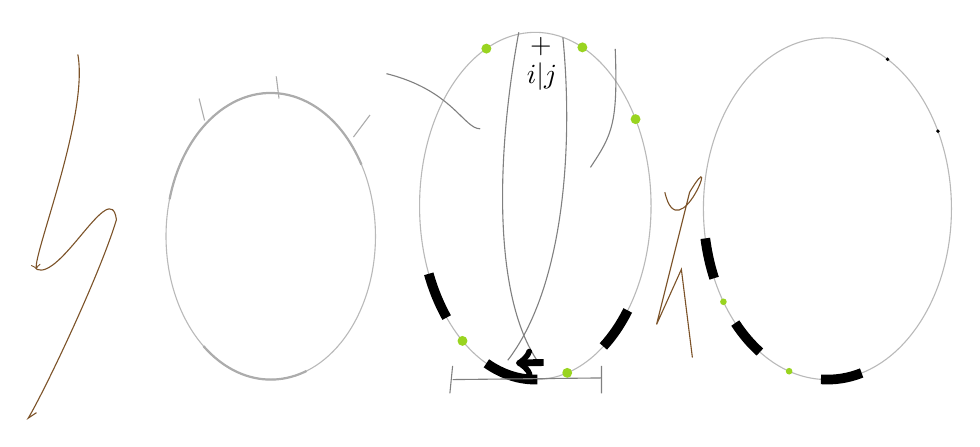
\begin{tikzpicture}[scale=.7]
\draw[gray!55] (0,0) ellipse (1.9 and 2.6);
\draw[gray!65,thick] (30:1.9 and 2.6) arc (30:165:1.9 and 2.6) (230:1.9 and 2.6) arc (230:290:1.9 and 2.6);
\draw[gray!65] (-1.2,2.1)--(-1.3,2.5) (.15,2.5)--(.1,2.9) (1.5,1.8)--(1.8,2.2);
\draw[brown!65!black,->] (-3.5,3.3)..controls (-3.3,2.2) and (-4.3,-.3)..(-4.25,-.6);
\draw[brown!65!black] (-4.25,-.6)..controls (-3.8,-.8) and (-2.9,1.1)..(-2.8,.3)..controls (-3.1,-.7) and (-4.1,-2.8)..(-4.4,-3.3)--(-4.25,-3.2);
\begin{scope}[shift={(4.8,.55)}]
\draw[gray!55] (0,0) ellipse (2.1 and 3.15);
\foreach \a in {30,66,115,231,286}{\fill[yellow!60!green] (\a:2.1 and 3.15) circle(.09);}
\foreach \a/\b in {203/220,245/271,306/323}{\draw[line width=3.5pt] (\a:2.1 and 3.15) arc (\a:\b:2.1 and 3.15);}
\draw[gray] (-.3,3.15)..controls (-.7,1) and (-.8,-1.7)..(.1,-2.9);
\draw[gray] (.5,3.06)..controls (.7,1) and (.5,-1.5)..(-.5,-2.8);
\draw[gray] (-2.7,2.4)..controls (-1.5,2.1) and (-1.3,1.4)..(-1,1.4);
\draw[gray] (1.45,2.85)..controls (1.5,1.5) and (1.4,1.3)..(1.0,.7);
\draw[gray] (-1.5,-3.15)--(1.2,-3.12) (-1.55,-3.4)--(-1.5,-2.9) (1.2,-3.4)--(1.2,-2.9);
\draw[<-,line width=2.5pt] (-.35,-2.85)--(.15,-2.84);
\node at (.1,2.9) {$+$};\node at (.12,2.35) {$\unsure{i|j}$};
\end{scope}
\begin{scope}[shift={(10.1,.5)}]
\draw[gray!55] (0,0) ellipse (2.25 and 3.1);
\foreach \a/\b in {190/204,222/237,267/286}{\draw[line width=3.5pt] (\a:2.25 and 3.1) arc (\a:\b:2.25 and 3.1);}
\foreach \a in {213,252}{\fill[yellow!60!green] (\a:2.25 and 3.1) circle(.06);}
\fill (61:2.25 and 3.1) circle(.035) (27:2.25 and 3.1) circle(.035);
\draw[brown!65!black] (-2.95,.3)..controls (-2.7,-.8) and (-1.9,1.3)..(-2.5,.3)--(-3.1,-2.1)--(-2.65,-1.1)--(-2.45,-2.7);
\end{scope}
\end{tikzpicture}}
\mspage{56}
\scanpage{58}
% E: text|upper left date|3.1.84
3.1.84
\deleted{
% E: text|upper left title three lines|Transport parallèle le long
Transport parallèle le long d'un demi-tour, \deleted{\unsure{au le|au}} le long d'une portion ultra \deleted{\unsure{singulière de polyg.}} \inserted{supersingulière}
% E: display|upper left boxed formula|lambda(t)
\[\boxed{\lambda(t)=t-(n-1)}\]
% E: text|left upper middle|NB Le pgcd
\uline{NB} Le pgcd de $n-1$ et de $2n$ est $1$ si $n$ pair, $2$ si $n$ impair.
% E: text|left middle introductory sentence|Donc on voit que l'image
Donc on voit que l'image de
% E: diagram|left middle|pi1(X) to D2n
\diagram{\begin{tikzcd}
\pi_1(X)\arrow[r] & \deleted{\unsure{\mathbb Z}}\mathbb D_{2n}
\end{tikzcd}}
% E: text|left middle image and index|a une image qui contient
 a une image qui contient $\mathbb D_{2n}^{+}\inserted{\unsure{{}\simeq\mathbb Z/2n\mathbb Z}}$ si $n$ pair (donc cette image est d'indice $1$ ou $2$) \deleted{ou bien elle} \inserted{et elle contient $\mathbb Z/n\mathbb Z$ si $n$ impair} (donc elle est tjrs d'indice $1,2$ ou $4$).
% E: text|left lower middle cutting and translation|Si on prend le découpage
\deleted{\unsure{Cela ne serait vrai}} Si on prend le \unsure{découpage} $\widetilde X$ de $X$ suivant les composantes supersingulières de $K$, on trouve dans l'image de
% E: diagram|left lower|pi1(X tilde) to D2n
\diagram{\begin{tikzcd}
\pi_1(\widetilde X)\arrow[r] & \mathbb D_{2n}
\end{tikzcd}}
% E: text|left lower|la translation
la translation
% E: display|left bottom|t to lambda prime(t)
\[t\longrightarrow\lambda'(t)=t-2(n-1).\]
% E: text|left bottom final two lines|Or le pgcd
Or le pgcd de $2(n-1)$ et \unsure{$n$|$2n$} est \unsure{un div. tjrs $2$|ici tjrs $2$}.
Donc l'image contient tjrs $\mathbb Z/n\mathbb Z$, d'indice $4$
% E: text|right top continuation|le quotient étant D2
(le quotient étant $\mathbb D_2\simeq\mathbb F_2\times\mathbb F_2$)
% E: text|right upper paragraph|Ceci ne nous dit rien
Ceci ne nous dit \inserted{rien} sur l'image de $\pi_1(X)$, $\pi_1(\widetilde X)$ dans $\mathbb D_2$, et en particulier sur son image dans $\pm1$, \inserted{\unsure{par}} composée avec
% E: diagram|right upper middle|D2n to plus or minus 1
\diagram{\begin{tikzcd}
\mathbb D_{2n}\arrow[r,"\chi"] & \pm1
\end{tikzcd}}
% E: text|right middle and lower|On a l'impression
On a l'impression que pour avoir des informations, il faut faire pivoter une \unsure{p.r.|por.} autour d'un sommet de $\uline{\Sigma}$ et faire ainsi un cycle et voir l'effet produit. On va faire un demi-tour, à partir d'une position supersingulière disons, par transport parallèle l'orientation de la position supersingulière aura changé, et \deleted{$\unsure{\chi}$} $\chi(\lambda)$ sera égal : $+1$ si le nb total des ``pas'' pour revenir au pt de départ est \uline{impair}; $-1$ dans le cas contraire. Donc on devrait pouvoir le faire en un nb \uline{pair} de pas !
}
% E: margin note|diagonal upper middle|Toute la partie
\margin{\unsure{Toute la partie combinée !|Toute la partie combinatoire !}}
% E: margin note|diagonal centre lower dated 4.1|Attention
\margin{4.1. Attention ! Ces \unsure{positions|portions} sont exclues dans le jeu des $\operatorname{Pol}(\unsure{D|CD})$}
% E: margin note|diagonal bottom centre|cf notes du 4.1
\margin{\unsure{Génial|Général} cf notes du 4.1.}
\mspage{57}
\scanpage{59}
\deleted{
% E: text|upper left first paragraph|Par une petite modification
Par une petite modification de ce parcours, on montre alors que non seulement $\pi_1(X)\longrightarrow\pm1$, mais aussi $\pi_1(\widetilde X)\longrightarrow\pm1$ est surjectif; \unsure{je dis|je dirai} dans le cas $n$ pair, cela implique que $\pi_1(\unsure{\widetilde X|\widetilde{\widetilde X}})\longrightarrow\mathbb D_{2n}$ est surjectif (mais peut-être pas $\pi_1(\widetilde X)\longrightarrow\mathbb D_2$ ?)
% E: text|left middle heading|Calcul de la parité
Calcul de la parité du nb d'opérations élémentaires pour passer de $(D_i^s,u)$ à $(D_i^s,-u)$.
% E: text|middle introductory line|Le nb d'opérations
Le nb d'opérations est égal à :
% E: display|middle three lines|2(nb de sommets à balayer)
\[
\begin{gathered}
2(\text{nb de sommets à balayer})\\
+2(\text{nb de droites par dessus lesquelles}\ \text{balaye.})\\
+1\ (\text{décollage})+1\ (\text{atterrissage})
\end{gathered}
\]
% E: drawing|left middle beside count|horizontal line point s upward arrow
\figure{\begin{tikzpicture}[scale=.8]
\draw (-1.5,0)--(-.18,0) (.2,0)--(2.9,0);\fill (0,0) circle(.06);\node[below] at (0,0) {$s$};\draw[->] (.8,.2)--(.7,.85);
\end{tikzpicture}}
% E: margin note|middle right attached by brace to count|NB chaque droite
\margin{NB chaque droite par dessus laquelle on balaye compte comme un \unsure{demi} sommet par lequel on balayerait}
% E: text|lower left exclamation|merveilleux
merveilleux, c'est toujours pair !
% E: text|lower left cancelled opening|En fait par transport parallèle
\deleted{En fait, par transport parallèle, on trouve \unsure{bien ce pt.}}
% E: text|bottom left qualification|A vrai dire
A vrai dire, le raisonnement \unsure{est conclusif|n'est conclusif} parce que il faut \unsure{se placer ici} dans le cas des $\unsure{L|X}$ qui n'ont pas de faces supersingulières (pas des ``bandes supersingulières'') car celles-ci sont d'indice $2(n-1)$, non $2n$. Donc il vaut mieux
% E: text|right top continuation|partir d'une portion
partir d'une position proche de $D_i$ passant par $s$, par un petit pivotement autour de $s$.
% E: text|right upper middle revised count|Maintenant toute droite
Maintenant, toute droite à franchir compte comme \uline{une seule} opération; \unsure{du lg|de là}, et chaque droite \inserted{passant par $s$} \deleted{franchie} \inserted{est} franchie une fois et une seule. Donc le nb correct d'opérations est
% E: display|right middle two lines|2(nb de sommets non liés en s)+ordre de s
\[
\begin{gathered}
2(\text{nb de sommets non}\ \uline{\text{\unsure{ligués|liés}}}\ \text{en }s)\\
+\text{ordre de }s.
\end{gathered}
\]
% E: text|right lower conclusion|donc l'image du circuit
 donc l'image du circuit dans $\pm1$ est $-1$ ou $+1$, suivant que l'ordre \deleted{\unsure{de}} $\nu(s)$ de $s$ est pair ou impair.
Si donc il y a au moins un sommet simple, on est \unsure{sûr que l'on a bien} $\pi_1(\unsure{\widetilde X|\widetilde{\widetilde X}})\longrightarrow\pm1$ surjectif, et encore $\pi_1(\widetilde X)\longrightarrow\unsure{\pm1|\mathbb D_{2n}}$ surj.
}
\mspage{58}
\scanpage{60}
% E: text|upper left first paragraph|Par contre si on fait un tour complet
Par contre, si on fait un tour complet, de façon à revenir à l'orientation de départ de $D$, alors \unsure{évidemment} (c'est le carré du \unsure{lent|petit} demi-tour) on trouve \deleted{\unsure{que alors que ce}} \inserted{un transport parallèle}
% E: diagram|upper left last line of first paragraph|Pol(D) to Pol(D)
\diagram{\begin{tikzcd}\operatorname{Pol}(D)\arrow[r] & \operatorname{Pol}(D)\end{tikzcd}}
% E: text|upper left continuation|qui conserve l'orientation
qui conserve l'orientation.
\deleted{
% E: text|left middle second paragraph|Notons aussi
Notons aussi que \deleted{\unsure{le nb}} pour le ``\unsure{lent|petit} demi-tour autour de $s$'', \deleted{\unsure{comme}} \inserted{quand} le nb de pas est pair, alors le résultat du transport parallèle sur les polygônes des \unsure{positions|portions} donne, sur l'orientation le $=$ résultat que le transport parallèle ordinaire de l'orientation. Cela signifie que l'orientation change \deleted{\unsure{par}} le long de ce \unsure{CCt|Cct}, si $\nu(s)$ pair.
% E: text|left lower paragraph also obliquely cancelled|Si nu(s) impair
Si $\nu(s)$ impair, alors le résultat sur $\operatorname{Pol}(\unsure{D})$, et via transport ordinaire, c'est \deleted{\unsure{pr}} le $=$. \deleted{\unsure{donc}} \inserted{comme} l'orientation est \uline{conservée} par transport parallèle, elle ne l'est pas par transport ordinaire --- donc en tous cas cette dernière change
}
\deleted{
% E: text|right upper continuation|ceci vaut chaque fois
ceci vaut chaque fois qu'on a un circuit fermé sur $X$ (circuit composé de faces) tel que le transport par. ordinaire change l'orientation de \deleted{\unsure{D}} la position \unsure{relative|rectiligne} $D$.
% E: text|right upper middle revised orientation assertion|Alors l'orientation
\deleted{Que le nb d'opérations soit pair \unsure{ne paraît}} \inserted{Alors l'orientation de $X$ change parce que} \unsure{le nb des pas élémentaires est pair}.
% E: text|right middle counting sweeps|Balayer au dessus
Balayer au dessus d'un pt compte comme $2$, balayer au dessus d'une \unsure{p.r.|pce} supersingulière compte comme $1$.
}
% E: text|right lower new assertion|Voilà enfin une façon de voir
Voilà enfin une façon de voir que $\pi_1(\unsure{\widetilde X|\widetilde{\widetilde X}})\longrightarrow\mathbb D_{2n}$ est surjectif.
% E: text|right lower before drawing|On part avec une \unsure{p.r.|por.}
On part avec une \unsure{p.r.|por.} \deleted{\unsure{D D}} \inserted{$D$} proche d'une \unsure{p.r.|por.} supersingulière $D_0$,
% E: drawing|bottom right|green sigmoid D red D0 two red verticals s s prime a
\figure{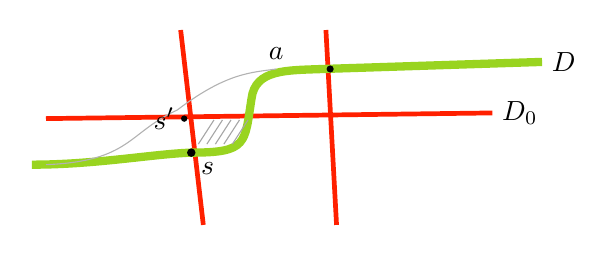
\begin{tikzpicture}[x=.9cm,y=.9cm]
\draw[red!75!orange,line width=1.7pt] (-2.7,0)--(3.6,.08) (-.8,1.25)--(-.48,-1.5) (1.25,1.25)--(1.4,-1.5);
\draw[yellow!60!green,line width=3pt] (-2.9,-.65)..controls (-2,-.65) and (-1.2,-.5)..(-.65,-.48)..controls (.15,-.48) and (.1,-.35)..(.2,.28)..controls (.25,.7) and (.7,.68)..(1.2,.7)--(4.3,.8);
\draw[gray!60] (-2.7,-.65)..controls (-1.5,-.6) and (-1.55,-.2)..(-.85,.12)..controls (-.15,.65) and (.2,.65)..(.55,.7);
\foreach \x in {-.55,-.43,-.31,-.19,-.07}{\draw[gray!70] (\x,-.36)--({\x+.22},-.02);}
\fill (-.65,-.48) circle(.06) (-.75,0) circle(.045) (1.31,.7) circle(.05);
\node[below right] at (-.65,-.48) {$s$};\node[left] at (-.75,0) {$s'$};\node[above] at (.55,.7) {$a$};\node[right] at (4.3,.8) {$D$};\node[right] at (3.6,.08) {$D_0$};
\end{tikzpicture}}
\mspage{59}
\scanpage{61}
\deleted{
% E: text|upper left continuation from previous sheet|d'où un côté privilégié
\deleted{\unsure{deux choix}} d'où un côté privilégié $a$ de $D$ (celui qui rencontre $D_0$), dont je choisis une extrémité $s$, de façon à avoir un repère.
% E: text|left upper middle specialization and half-turn|Je spécialise D en D prime
Je spécialise $D$ en $D'$ vers le \deleted{\unsure{F}} \inserted{sommet} $s'$ le plus proche de $s$, je fais un demi-tour par $s$, et je reviens à $D$, --- un nb pair d'opérations, qui change l'orientation de $D$, \uline{et transforme $s$ en $\unsure{s|s'}$} --- donc c'est la symétrie par \unsure{rapport à} $s$. Si on fait
}
% E: text|left lower new date and definition|4.1 Pour tout chemin
4.1. Pour tout \deleted{\unsure{bout}} chemin \inserted{$c$} combinatoire sur $\Gamma$ --- i.e. chemin formé avec des faces $\overline F_D$ de $(X,K)$, reliant la face $F=\overline F_D$ à une $F'=\overline F_{D'}$, on trouve un iso. de ``transport parallèle''
% E: diagram|left lower|Pol(c) Pol(F) dash Pol(F prime)
\diagram{\begin{tikzcd}
\operatorname{Pol}(c):\quad\operatorname{Pol}(F)\arrow[r,dash] & \operatorname{Pol}(F')
\end{tikzcd}}
% E: text|left bottom intrinsic geometry paragraph|qui du pt de vue
qui du pt de vue de la géométrie intrinsèque de $(X,K,S_K)$ s'interprète par composition successive de ``réflexions'' le long des côtés de réflexion qui interviennent \unsure{au cours sur $c$|au cours de $c$}.
% E: text|right top|L'effet de Pol(c) sur les orientations
L'effet de $\operatorname{Pol}(c)$ sur les orientations
% E: diagram|right upper orientation sets|omegaX(c) omega(F) to omega(F prime)
\diagram{\begin{tikzcd}
\underline\omega_X(c):\quad\underline\omega(F)\simeq\underline\omega(D)\arrow[r] & \underline\omega(F')\simeq\underline\omega(D')
\end{tikzcd}}
% E: text|right upper middle|est aussi l'effet
est aussi l'effet sur l'orientation des \unsure{p.r.|p.v.} par transport parallèle --- donc est indépendant de la parité du nb de pas dans le chemin $c$ ! Si on a un circuit \deleted{$\unsure{\ell}$} $\ell=c$ i.e. $F=F'$ --- on a
% E: diagram|right middle|fundamental group to automorphisms to sign
\diagram{\begin{tikzcd}[column sep=large]
\pi_1(X,F_D)\arrow[r] & \underset{{}\simeq\mathbb D_{2n}}{\operatorname{Aut}(\operatorname{Pol}(D))}\arrow[r,"\substack{\text{effet sur}\\\text{orientation}}"] & \pm1
\end{tikzcd}}
% E: text|right middle introducing character|on désignera par chiX
on désignera par $\chi_X$ le caractère composé
% E: display|right middle character|chiX pi1(X FD) to sign
\[\chi_X:\pi_1(X,F_D)\longrightarrow\pm1\]
% E: text|right middle lower sign interpretation|donc pour un chemin
donc pour un chemin $\ell$, on aura $\chi_{\unsure{X}}(\ell)=+1$ ou $-1$ suivant que par transport parallèle l'orientation de $D$ aura ou non changé. \deleted{\unsure{On}}
% E: text|right lower two other characters|On a deux autres caractères
On a deux autres caractères $\chi_s$ et $\chi_a$ (\unsure{colorations|interversions} sommets et arêtes) en associant à chaque face $F_D$ les deux ensembles à deux éléments
% E: display|right bottom first two-element set|epsilon s(F) epsilon s(D)
\[
\begin{aligned}
\epsilon_s(\unsure{F|D})=\epsilon_s(D)={}&\text{un des }\inserted{\text{deux}}\ n\text{-gones}\\
&\text{inscrits dans }\unsure{\Pi_0|\pi_0}(D)=\operatorname{Pol}(F),
\end{aligned}
\]
% E: display|right bottom second two-element set|epsilon a(D) epsilon a(F)
\[
\begin{aligned}
\epsilon_{\unsure{a|s}}(\unsure{D|F})=\epsilon_a(F)={}&\text{un des deux }n\text{-gones}\\
&\text{circonscrits dans }\operatorname{Pol}(D)=\operatorname{Pol}(F)
\end{aligned}
\]
\mspage{60}
\scanpage{62}
% E: text|printed top seven lines|HASP373 STARTED
\texttt{\unsure{\$HASP373} STARTED - INIT 2 - CLASS 1 - SYS E333}\par
\texttt{IEF236I ALLOC. FOR CRAY2}\par
\texttt{IEF142I CRAY2 - STEP WAS EXECUTED - COND CODE 0000}\par
\texttt{IEF373I STEP /\qquad / START 82229.0906}\par
\texttt{IEF374I STEP /\qquad / STOP 82229.0906 CPU 0MIN 00.01SEC SRB 0MIN 00.00SEC VIRT 8K SYS 200K}\par
\texttt{IEF375I JOB /CRAY2\qquad / START 82229.0906}\par
\texttt{IEF376I JOB /CRAY2\qquad / STOP 82229.0906 CPU 0MIN 00.01SEC SRB 0MIN 00.00SEC}
% E: diagram|upper left handwritten first line|F=FD to FDprime=Fprime
\diagram{\begin{tikzcd}
F=F_D\arrow[r] & F_{D'}=F'
\end{tikzcd}}
% E: diagram|left three rows of orientation objects|omega FD omega F omega D
\diagram{\begin{tikzcd}[row sep=large,column sep=huge]
\omega(F_D)\arrow[r,"\alpha\ \text{transport parallèle}","\unsure{\text{c.-à-d. via les }\operatorname{Pol}(D)}"']\arrow[d,phantom,"{\rotatebox{90}{$\simeq$}}" description] & \omega(F_{D'})\arrow[d,phantom,"{\rotatebox{90}{$\simeq$}}" description]\\
\omega(\unsure{F|\overline F})\arrow[r,"\beta\ \text{transport de}","\text{l'orientation sur }X"']\arrow[d,phantom,"{\rotatebox{90}{$\simeq$}}" description] & \omega(F')\arrow[d,phantom,"{\rotatebox{90}{$\simeq$}}" description]\\
\omega(D)\arrow[r,"\alpha'\ \text{transport parallèle}"] & \omega(D')
\end{tikzcd}}
% E: drawing|upper middle pencil sketch|two nearly tangent loops
\figure{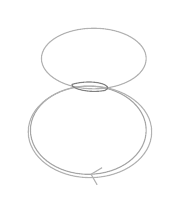
\begin{tikzpicture}[scale=.7]
\draw[gray!60] (.1,1.3) ellipse (.95 and .55);
\draw[gray!70] (0,0) ellipse (1.05 and .8);
\draw[gray!60] (.03,-.03) ellipse (1.12 and .83);
\draw[gray] (-.3,.83)..controls (.1,.95) and (.5,.8)..(.3,.72)..controls (0,.67) and (-.3,.75)..(-.3,.83);
\draw[gray!60] (.05,-.8)--(.25,-.68) (.05,-.8)--(.16,-.99);
\end{tikzpicture}}
% E: drawing|right middle|sigmoid line crossed by three verticals
\figure{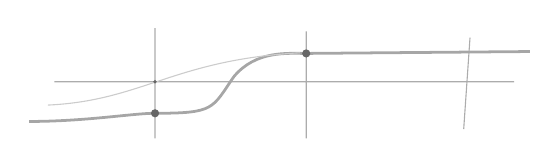
\begin{tikzpicture}[scale=.8]
\draw[gray!65] (-3,0)--(4.3,0) (-1.4,-.9)--(-1.4,.85) (1,-.9)--(1,.8) (3.5,-.75)--(3.6,.7);
\draw[gray!70,line width=1pt] (-3.4,-.63)..controls (-2.5,-.63) and (-1.75,-.5)..(-1.4,-.5)..controls (-.45,-.5) and (-.5,-.43)..(-.15,.08)..controls (.2,.5) and (.7,.45)..(1,.45)--(4.55,.48);
\draw[gray!40] (-3.1,-.37)..controls (-1.6,-.3) and (-1.1,.35)..(.9,.46);
\fill[gray!80!black] (-1.4,-.5) circle(.065) (1,.45) circle(.065) (-1.4,0) circle(.03);
\end{tikzpicture}}
% E: display|middle lower relation between alpha and beta|alpha=alpha prime
\[\alpha=\alpha'\qquad\beta=\alpha,\alpha'\quad\text{ssi. nb d'opérations }\inserted{N}\text{ est pair}\]
% E: display|lower example line|ex F=FDprime
\[\text{ex }F=F_{D'},\quad\alpha=\alpha'=-1\qquad\text{alors }\beta=-1\quad\text{ssi }\deleted{\unsure{nb}}\ N\text{ pair}\]
% E: text|lower left unfinished conclusion|donc
 donc
\mspage{61}
\scanpage{63}
\mspage{62}
% E: text|upper left|et tout chemin
et tout chemin \inserted{$c$} définit des iso. d'ens à deux éléments
% E: diagram|upper left|omega epsilon_s epsilon_a
\diagram{\begin{tikzcd}[column sep=large,row sep=small]
\underline\omega(\unsure{F|D})\simeq\underline\omega(D) \arrow[r,"\underline\omega_X(c)"] & \underline\omega(\unsure{F'|D'})\simeq\underline\omega(D')\\
\varepsilon_s(F)=\varepsilon_s(D) \arrow[r] & \varepsilon_s(F')\simeq\varepsilon_s(D')\\
\varepsilon_a(F)\unsure{\simeq|=}\varepsilon_a(D) \arrow[r] & \varepsilon_a(F')\simeq\varepsilon_a(D')
\end{tikzcd}}
% E: text|left upper middle|Ces ens. ne sont pas indépendants
Ces ens. ne sont pas indépendants, chaque paire des deux détermine le troisième, par la relation
% E: display|left upper middle|omega(F) epsilon_s(F) wedge epsilon_a(F)
\[\underline\omega(F)\simeq\varepsilon_s(F)\wedge\varepsilon_a(F)\]
% E: text|left middle|et les deux relations
et les deux relations \unsure{circulaires|analogues} équivalentes.

Au niveau des caractères correspondants sur $\pi_1(X,F)$, cela donne
% E: diagram|left middle|chi_X(F)=chi_s(F)chi_a(F)
\diagram{\begin{tikzcd}[row sep=small]
\boxed{\chi_X(F)=\chi_s(F)\chi_a(F)} \arrow[d,phantom,"\rotatebox{90}{$=$}" description]\\
\chi_X(D)=\chi_s(D)\chi_a(D) \arrow[d,phantom,"\rotatebox{90}{$=$}" description]\\
\underline\omega(D)
\end{tikzcd}}
% E: text|left middle|ou de façon plus symétrique
ou de façon plus symétrique
% E: display|left middle|chi_X(F)chi_s(F)chi_a(F)=1
\[\chi_X(F)\chi_s(F)\chi_a(F)=1.\]
% E: text|lower left|En plus de ces trois caractères
En plus de ces trois caractères, il y en a deux autres, $\chi_{\mathcal X}={}$caractère d'\unsure{orientabilité|orientation} de $\mathcal X$ (ne dépendant pas de la structure cellulaire), et $\chi_c$ (``combinatoire''), qui est donné par la parité \inserted{\unsure{du tout|de tout}}. Le système local \deleted{\unsure{associé est les|associé les}} \inserted{correspondant est défini par les} $\underline\omega(F)$, mais avec des identifications de transition \uline{opposées} à celles données par \deleted{\unsure{identifications}} le transport parallèle sur $X$
% E: margin note|diagonal centre with arrow to parity phrase|Attention dans le
\margin{Attention, dans le \unsure{pointé|point}, \uline{est faux}, il faut compter pour \uline{deux} le franchissement d'un côté \unsure{except\textsuperscript{l}|except.} (qui \unsure{accroche|accrocherait}), \unsure{soit décomposer en|décomposé en} \uline{deux} opérations.}
% E: text|upper right|défini par les omega_X(c)
défini par les $\underline\omega_X(c)$ --- donc on aura
% E: display|upper right|omega_Xcal(c)=p(c)omega_X(c)
\[\underline\omega_{\mathcal X}(c)=\unsure{\mathrm{par}|p}(c)\omega_X(c)\]
% E: text|upper right|où p(c) désigne la parité
\unsure{où} $\unsure{\mathrm{par}|p}(c)$ désigne la parité de $c$.
\deleted{En prenant} Le système local associé à $\chi_c$ a \deleted{formé de} comme fibres les ens. triviaux $\{\pm1\}$, mais les morphismes de transition donnés par les $\unsure{\mathrm{par}|p}(c)$.

On en a donc
% E: display|right middle|chi_Xcal=chi_o chi_c
\[\boxed{\chi_{\mathcal X}=\chi_{\unsure{o|X}}\chi_c}\]
% E: margin note|right edge alongside boxed formula|On a chi_c=1
\margin{On a $\chi_c=1$ \unsure{cf p\textsuperscript{o}|si $\Gamma$} \unsure{suivante!}}
% E: text|right middle|Donc compte tenu de ces relations
Donc, compte tenu de ces relations, on dispose de trois caractères fondamentaux \inserted{\unsure{privilégiés}}, que je choisis
% E: display|right lower middle|chi_X chi_s chi_c
\[\chi_X,\chi_s,\chi_c\]
% E: text|right lower middle|donc les deux autres sont
\unsure{donc} les deux autres sont
% E: display|right lower middle|chi_a=chi_X chi_s
\[\chi_a=\chi_X\chi_s\quad\text{et surtout}\quad\chi_{\mathcal X}=\chi_X\chi_c\]
% E: text|bottom right|Il y a lieu d'expliciter
Il y a lieu d'expliciter les valeurs des caractères précédents, si faire se peut, ainsi que celles des représentations
% E: display|bottom right|u pi_1(X F_D) to Aut(Pol(D))
\[u:\pi_1(X,F_D)\longrightarrow\operatorname{Aut}(\operatorname{Pol}(D)),\]
\scanpage{64}
\mspage{63}
% E: text|upper left|Pour les circuits fondamentaux
Pour les circuits fondamentaux sur $X$, \unsure{qui est|qui sont} de deux espèces

 a) \inserted{\uline{demi}} Circuit autour d'une \deleted{\unsure{droite}} \inserted{composante} exceptionnelle de $K$ (en la traversant une fois), soit $\ell_{D_i}$ le circuit correspondant à la pseudodrte $D_i\in\Sigma$. On trouve
% E: display|left upper middle|u(ell_D_i) translation par n-1
\[u(\vec\ell_{D_i})=\text{translation par }n-1\]
% E: text|left middle|dans le sens de l'orientation
(dans le sens de l'orientation de la portion \unsure{rect\textsuperscript{g}|rel.} $D$ voisine de $D_i$), valeurs des caractères fondamentaux
% E: display|left middle|chi_X(ell_D_i)=+1
\[\chi_X(\ell_{D_i})=+1,\quad\chi_s(\ell_{D_i})=\deleted{\unsure{+1}}(-1)^{n-1},\quad\deleted{\chi_c(\ell_{D_i})=1}\]
% E: text|lower left|b Demi-circuit autour d'un pt
b) Demi-circuit autour d'un pt de $X$ (qui peut être soit dans une face, soit dans un côté, soit \inserted{être} un sommet). La \deleted{point} \unsure{fibre} de ce point dans $\operatorname{Pol}(D)$ reste fixe par $u(\ell)$, qui est de signe $-1$, donc on trouve toutes les symétries, donc
% E: drawing|left margin beside b|double vertical emphasis
\figure{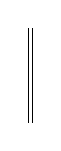
\begin{tikzpicture}[x=.2cm,y=.4cm]\draw (0,0)--(0,3);\draw (.25,0)--(.25,3);\end{tikzpicture}}
% E: display|lower left|u_D pi_1(X F_D) to Aut(F_D)
\[u_D:\pi_1(X,F_D)\longrightarrow\operatorname{Aut}(F_D)\]
% E: text|bottom left|est surjectif ouf
est \uline{surjectif}. ouf!
% E: text|upper right|Il semble que le caractère chi_c soit trivial
$*$ Il semble que le caractère $\chi_c$ soit \uline{trivial}! En effet, si pour une p.r. $D$ donnée, on désigne par $\mathrm{sing}_D$ (``singularité de $D$'') le nb de sommets de $\Sigma$ qu'elle contient, je dis que pour un chemin $c$ qui va de $D$ en $D'$, on a
% E: display|right upper middle|par c congruent sing_D' minus sing_D
\[\unsure{\mathrm{par}}\,c\equiv\mathrm{sing}_{D'}-\mathrm{sing}_D\qquad(2)\]
% E: text|right middle|donc parité paire si D=D'
(donc parité = \uline{paire} si $D=D'$!)
On est ramené au cas où $c$ est de longueur $1$, auquel cas cette formule est triviale. (en se rappelant que pour le franchissement \deleted{d'une \unsure{di.}} un ``balayage'' au dessus d'une \deleted{\unsure{droite}} $D_i\in\Sigma$, la parité est $2$.

Donc finalement, \uline{on trouve}
% E: display|lower right|chi_Xcal=chi_X
\[\boxed{\chi_{\mathcal X}=\chi_X}\]
% E: text|bottom right|il n'y a pas d'autres caractères
il n'y a pas d'autres caractères rigides que ceux provenant de $\mathbb D_2$!
\scanpage{65}
\mspage{64}
% E: text|top left|3.1.84
3.1.84
% E: drawing|upper left|Delta_D' D' a a' s
\figure{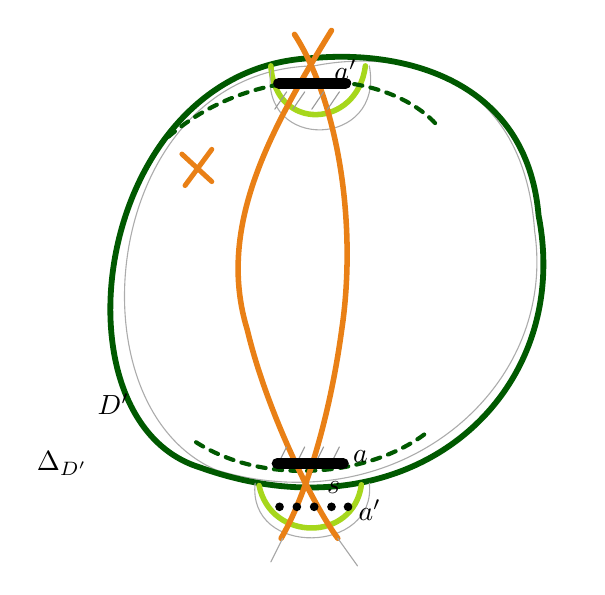
\begin{tikzpicture}[x=1cm,y=1cm,line cap=round,line join=round]
\draw[gray!65] (0,2.7) .. controls (-2.7,2.65) and (-3.15,-1.6) .. (-1.25,-2.43) .. controls (1,-3.12) and (3.1,-1.45) .. (2.8,.6) .. controls (2.65,2.7) and (1,2.9) .. (0,2.7);
\draw[green!35!black,line width=2.1pt] (0,2.8) .. controls (-2.8,2.7) and (-3.4,-1.8) .. (-1.45,-2.4) .. controls (1.2,-3.35) and (3.3,-1.5) .. (2.85,.8) .. controls (2.7,2.55) and (1.1,2.9) .. (0,2.8);
\draw[yellow!65!green,line width=2pt] (-.55,2.7) .. controls (-.5,1.85) and (.55,1.9) .. (.65,2.7);
\draw[gray!65] (-.55,2.65) .. controls (-.7,1.6) and (.9,1.65) .. (.7,2.7);
\draw[green!35!black,line width=1.5pt,dashed] (-1.85,1.8) .. controls (-.7,2.8) and (1,2.65) .. (1.6,1.9);
\draw[green!35!black,line width=1.5pt,dashed] (-1.5,-2.08) .. controls (-.6,-2.65) and (.7,-2.5) .. (1.4,-1.98);
\draw[yellow!65!green,line width=2pt] (-.7,-2.63) .. controls (-.55,-3.35) and (.5,-3.35) .. (.6,-2.62);
\draw[gray!65] (-.75,-2.6) .. controls (-.85,-3.55) and (.8,-3.5) .. (.7,-2.6);
\draw[orange!65!brown,line width=2pt] (-.25,3.1) .. controls (.3,2.25) and (.55,.7) .. (.35,-.65) .. controls (.2,-1.75) and (-.1,-2.75) .. (-.42,-3.3);
\draw[orange!65!brown,line width=2pt] (.22,3.15) .. controls (-.55,1.9) and (-1.25,.65) .. (-.85,-.65) .. controls (-.6,-1.7) and (0,-2.9) .. (.3,-3.3);
\draw[gray!70] (-.4,-3.3)--(-.55,-3.6) (.3,-3.3)--(.55,-3.65);
\foreach \x in {-.35,-.12,.12,.32}{\draw[gray!80] (\x,2.37)--(\x-.15,2.15);\draw[gray!80] (\x,-2.14)--(\x-.12,-2.38);}
\draw[line width=4pt] (-.45,2.48)--(.4,2.48);
\draw[line width=4pt] (-.47,-2.35)--(.37,-2.35);
\foreach \x in {-.44,-.22,0,.22,.43}{\fill (\x,-2.9) circle (.055);}
\draw[orange!65!brown,line width=1.8pt] (-1.68,1.58)--(-1.3,1.23) (-1.64,1.18)--(-1.3,1.64);
\node at (.4,2.65) {$a'$};\node[right] at (.37,-2.26) {$a$};\node[right] at (.44,-2.94) {$a'$};\node[right] at (.04,-2.65) {$s$};\node at (-2.55,-1.6) {$D'$};\node at (-3.2,-2.35) {$\Delta_{D'}$};
\end{tikzpicture}}
% E: drawing|upper middle|Delta_D D b b' s
\figure{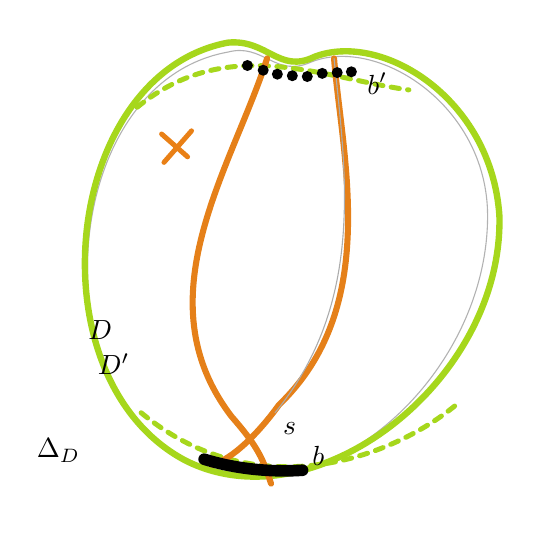
\begin{tikzpicture}[x=1cm,y=1cm,line cap=round,line join=round]
\draw[gray!60] (-.7,2.68) .. controls (-2.8,2.3) and (-3.1,-1.5) .. (-1.3,-2.5) .. controls (.4,-3.4) and (2.6,-1.5) .. (2.6,.6) .. controls (2.6,2) and (1.2,2.9) .. (.35,2.55) .. controls (-.1,2.35) and (-.25,2.8) .. (-.7,2.68);
\draw[yellow!65!green,line width=2.3pt] (-.7,2.8) .. controls (-2.8,2.4) and (-3.2,-1.45) .. (-1.25,-2.5) .. controls (.4,-3.35) and (2.8,-1.5) .. (2.75,.6) .. controls (2.65,2.1) and (1.25,2.95) .. (.4,2.62) .. controls (-.05,2.4) and (-.2,2.85) .. (-.7,2.8);
\draw[yellow!65!green,line width=1.8pt,dashed] (-1.85,1.98) .. controls (-.7,2.92) and (.5,2.35) .. (1.6,2.2);
\draw[yellow!65!green,line width=1.8pt,dashed] (-1.8,-1.9) .. controls (-.35,-3.1) and (1.35,-2.5) .. (2.2,-1.8);
\draw[orange!60!brown,line width=2.2pt] (-.2,2.6) .. controls (-.65,1.2) and (-1.8,-.45) .. (-.65,-1.95) .. controls (-.3,-2.35) and (-.25,-2.5) .. (-.15,-2.8);
\draw[orange!60!brown,line width=2.2pt] (.65,2.6) .. controls (.75,1.35) and (1.25,-.55) .. (-.05,-1.8) .. controls (-.3,-2.15) and (-.65,-2.5) .. (-.9,-2.56);
\draw[gray!65] (.65,2.6) .. controls (.8,1.15) and (1.05,-.5) .. (-.1,-1.9);
\foreach \x/\y in {-.45/2.51,-.25/2.45,-.07/2.4,.12/2.38,.31/2.37,.5/2.41,.69/2.42,.87/2.43}{\fill (\x,\y) circle (.07);}
\draw[line width=4.2pt] (-1,-2.49) .. controls (-.65,-2.6) and (-.2,-2.66) .. (.25,-2.63);
\draw[orange!65!brown,line width=1.8pt] (-1.54,1.64)--(-1.21,1.35) (-1.51,1.28)--(-1.16,1.68);
\node[right] at (.95,2.28) {$b'$};\node[right] at (.25,-2.45) {$b$};\node[right] at (-.12,-2.1) {$s$};\node at (-2.32,-.85) {$D$};\node at (-2.15,-1.28) {$\deleted{\unsure{D'}}$};\node at (-2.85,-2.38) {$\Delta_D$};
\end{tikzpicture}}
% E: text|below drawings across left two thirds|huit façons standart de recoller
huit façons ``standart'' de recoller $\Delta_D$ à $\Delta_{D'}$, \unsure{suiv\textsuperscript{t}} \deleted{\unsure{le}} \deleted{\unsure{une}} \unsure{isom.} choisi d'un des deux arcs de transition \inserted{$a,a'$} sur $\Delta_{D'}$, sur l'un des deux arcs privilégiés $b$ (de transition) et $b'$ (son antipodique) sur $\Delta_D$, deux choix pour chaque choix d'un couple dans $\{a,a'\}\times\{b,b'\}$. Donc huit façons à priori de construire une surface à bord \inserted{cellulaire} pour graphe $\Gamma_{\underline\Sigma}=\Gamma$, mais (sauf pour le \unsure{plongement} d'une courbe rouge, \unsure{différent}) il n'y a que quatre cas différents de surfaces, car \unsure{ceux} qu'on obtient pour un choix $(\alpha,\beta,\unsure{\rho|\sigma})$ \inserted{\unsure{iso. de recollement}} et $(\alpha',\beta',\sigma')$ (où $\alpha',\beta',\sigma'$ déduits en composant avec
% E: text|right column upper|les antipodismes
les antipodismes) sont can. isom. (ils correspondent à la $=$ circularisation de $\Gamma$, et les \unsure{$=$s|$=$} réflexions de transition pour les \unsure{or. loc.|syst. loc.} correspond. \unsure{du})

On peut \unsure{les supposer|donc supposer}, quitte à composer avec les antipodismes de part et d'autre, que $\beta=b$ --- ce qui revient à faire un choix où le sommet $s$ apparaît \deleted{\unsure{au}} au voisinage de l'arc de transition choisi, sur la surface recollée (au lieu qu'il soit rejeté aux antipodes, ce qui a l'air un peu idiot!)
% E: deletion|bottom right|P. cf les quatre dessins
\deleted{\unsure{P. cf} les quatre dessins (ou plutôt, les huit)} qui
\scanpage{66}
\mspage{65}
% E: deletion|upper left crossed through by diagonal strokes|sont en est qu'elles
\deleted{\deleted{\unsure{sont}} \unsure{en est qu'elles|ceux desquels} \unsure{il y a} une application canonique de la surface recollée dans $X$! \deleted{Si on recolle $b$ à $a$} \inserted{Non, c'est vrai pour $a'$}, \deleted{donc} \unsure{car}, pour $\alpha$ choisi, on choisira l'identification.}
% E: text|left upper middle|Si on veut une application naturelle
Si on veut une application naturelle de la surface recollée dans $X$, qui sur $\Delta_D$, $\Delta_{D'}$ se réduise au plongement canonique, il faut \inserted{(semble-t-il)} que $b$ et $\alpha$ se réalisent par le $=$ segment plongé dans $X$, ce qui \inserted{semble} imposer $\alpha=a'$. Mais si on convient de remplacer $\Delta_D$ par un disque \unsure{un plus petit|un peu petit} $\Delta_D^*$ \inserted{dont le bord} passe par $s$ (cf pointillé ci-contre), et déplacer \unsure{canoniquement} $b$ en $b^*$, et faire le recollement le long de $b^*$ plutôt que $b$, \deleted{donc} et pareil pour le disque $\Delta_{D'}$, (de façon à faire coïncider les images de $a$ et $a'$ dans $X$), on voit qu'on arrive à \deleted{\unsure{faire appliquer}} \inserted{\unsure{trouver}} une application de la surface recollée dans $X$, même en choisissant $\alpha=a$.
% E: drawing|lower left in paragraph|Delta_D star s b star
\figure{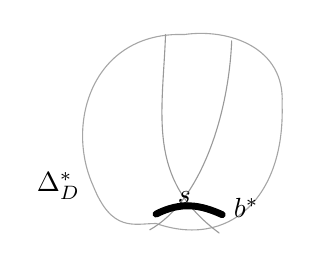
\begin{tikzpicture}[x=.8cm,y=.8cm,line cap=round]
\draw[gray!70] (0,1.8) .. controls (-1.45,1.85) and (-1.9,.4) .. (-1.45,-.6) .. controls (-1.15,-1.35) and (-.8,-1.2) .. (-.45,-1.2) .. controls (.7,-1.6) and (1.6,-.8) .. (1.55,.7) .. controls (1.6,1.6) and (.7,1.9) .. (0,1.8);
\draw[gray!80] (-.3,1.8) .. controls (-.35,.5) and (-.6,-.5) .. (.55,-1.35);
\draw[gray!80] (.75,1.7) .. controls (.7,.5) and (.25,-.85) .. (-.55,-1.3);
\draw[line width=2.5pt] (-.45,-1.05) .. controls (-.05,-.85) and (.25,-.9) .. (.6,-1.06);
\node at (0,-.78) {$s$};\node[right] at (.63,-.95) {$b^*$};\node at (-2,-.6) {$\Delta_D^*$};
\end{tikzpicture}}
% E: text|bottom left continuing top right|Le choix le plus naturel quand même
Le choix le plus naturel quand même (\deleted{\unsure{dans}} pt de vue application dans $X$), semblerait $\alpha=a'$. \unsure{Donc|Dans}, sur le terrain de dessin --- \uline{continuation} d'une rive par la suivante --- l'application $\mathcal X\longrightarrow X$ est une \uline{``immersion''}.
% E: drawing|right upper middle|two crossing orange arcs orientation arrows
\figure{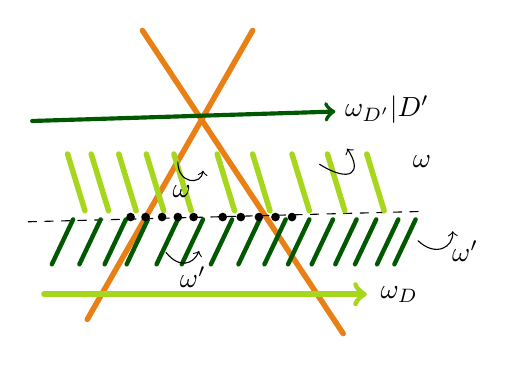
\begin{tikzpicture}[x=1cm,y=1cm,line cap=round,line join=round]
\draw[orange!65!brown,line width=2pt] (-1.3,2.15)--(1.25,-1.7);
\draw[orange!65!brown,line width=2pt] (.1,2.15)--(-2,-1.52);
\draw[green!35!black,line width=1.5pt,->] (-2.7,1)--(1.15,1.12);
\draw[yellow!65!green,line width=2pt,->] (-2.55,-1.2)--(1.55,-1.2);
\node[right] at (1.6,-1.2) {$\omega_D$};
\node[right] at (1.15,1.14) {$\unsure{\omega_{D'}|D'}$};
\draw[dashed] (-2.75,-.28)--(2.2,-.15);
\foreach \x in {-2.25,-1.95,-1.6,-1.25,-.9,-.35,.1,.6,1.05,1.55}{\draw[yellow!65!green,line width=2pt] (\x,.58)--(\x+.22,-.14);}
\foreach \x in {-2.45,-2.1,-1.78,-1.5,-1.12,-.8,-.43,-.08,.25,.55,.85,1.15,1.4,1.68,1.9}{\draw[green!35!black,line width=1.6pt] (\x,-.82)--(\x+.27,-.25);}
\foreach \x in {-1.45,-1.26,-1.05,-.85,-.65,-.28,-.05,.18,.39,.6}{\fill (\x,-.22) circle (.055);}
\draw[->] (-.85,.48) .. controls (-.85,.2) and (-.55,.18) .. (-.53,.37);\node at (-.8,.1) {$\omega$};
\draw[->] (.95,.45) .. controls (1.35,.2) and (1.5,.35) .. (1.3,.65);\node at (2.25,.48) {$\omega$};
\draw[->] (-1,-.67) .. controls (-.83,-.88) and (-.65,-.82) .. (-.58,-.65);\node at (-.66,-.98) {$\omega'$};
\draw[->] (2.2,-.52) .. controls (2.42,-.73) and (2.65,-.61) .. (2.64,-.4);\node at (2.8,-.65) {$\omega'$};
\end{tikzpicture}}
% E: text|right lower half|Dans cette optique la rive de D'
Dans cette optique \inserted{\unsure{donc}}, la rive de $D'$ i.e. l'arc sur $\partial\Delta_{D'}$ qui exprime l'orientation de \deleted{\unsure{spécialisation}} \inserted{\unsure{générisation}} vers $D$ est $a'$ --- i.e. celle qui ``fait face'' à la rive $a$, et non $a$ qui en est déduit par ``transport parallèle'' au cours de la déformation de spécialisation $D\longrightarrow D'$. Ce choix semble parfaitement naturel --- l'inverse,
\scanpage{67}
\mspage{66}
% E: text|upper left|c'est qu'il semble que sur la carte
c'est qu'il semble que sur la \unsure{carte|surface} $\mathcal X$ obtenue par recollement, on n'ait aucune interprétation des ``trous'' (ou sommets, quand on a bouché les trous) en termes de la géométrie de $\underline\Sigma$.
% E: margin note|left margin beside Il faudrait|emphasis mark
\margin{\unsure{*}}
% E: text|left middle and lower|Il faudrait quand même que j'y songe
Il faudrait quand même que j'y songe, pour voir si je \unsure{ne m'étais} pas mélangé les pinceaux\ldots{} Quand on a fait ce recollement, et qu'on suit par continuité une orientation donnée $\omega$ de $\Delta_D$ (définie par une or. $\omega_D$ de $D$) en passant de $\Delta_D$ dans $\Delta_{D'}$ via l'arc de transition, on trouve \deleted{que} une orientation $\omega'$ de $\Delta_{D'}$ qui induit sur $D'$ une orientation $\omega_{D'}$ qui est \uuline{opposée} de celle déduite par transport \deleted{\unsure{de la droite}} parallèle! Voilà donc rectifiée une erreur monumentale, commise dès le début!
% E: text|upper right|Venons-en à l'autre choix
Venons-en à l'autre choix qui donne lieu à $\mathcal X\longrightarrow X$, savoir $\alpha=a$. On est obligé ici de \unsure{porter|déporter} comme j'avais dit $\Delta_D,b$ et $(\Delta_{D'},a)$, pour faire se rencontrer $b$ et $a$ dans $b^*\sim a^*\subset X$. On trouve la figure
% E: drawing|right middle|omega'=-omega delta omega_D omega_D'
\figure{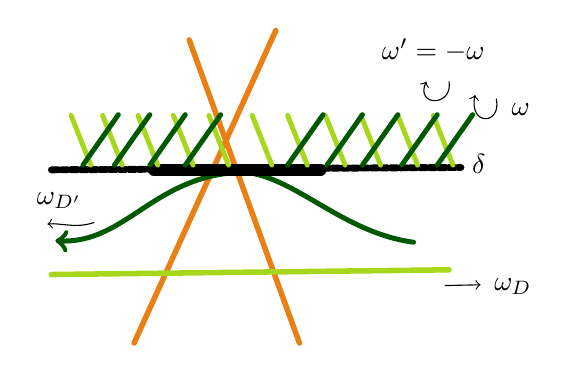
\begin{tikzpicture}[x=1cm,y=1cm,line cap=round,line join=round]
\draw[orange!65!brown,line width=2pt] (-.85,1.9)--(.55,-1.95);
\draw[orange!65!brown,line width=2pt] (.25,2.02)--(-1.55,-1.95);
\draw[green!35!black,line width=1.8pt,<-] (-2.55,-.65) .. controls (-1.65,-.7) and (-1.3,.2) .. (-.15,.22) .. controls (.5,.16) and (1.1,-.55) .. (2,-.67);
\draw[->] (-2.06,-.42)..controls (-2.3,-.5) and (-2.48,-.42)..(-2.65,-.44);
\node[above] at (-2.5,-.37) {$\omega_{D'}$};
\draw[yellow!65!green,line width=2pt] (-2.6,-1.08)--(2.45,-1.02);
\draw[->] (2.4,-1.22)--(2.85,-1.21);\node[right] at (2.9,-1.23) {$\omega_D$};
\draw[densely dotted,line width=2.5pt] (-2.6,.25)--(2.6,.28);
\draw[line width=4.2pt] (-1.3,.25)--(.82,.25);
\foreach \x in {-2.2,-1.8,-1.35,-.9,-.45,.1,.55,1.03,1.48,1.95,2.4}{\draw[yellow!65!green,line width=1.8pt] (\x-.15,.94)--(\x+.1,.31);}
\foreach \x in {-2.2,-1.8,-1.35,-.9,.4,.9,1.35,1.85,2.3}{\draw[green!35!black,line width=1.8pt] (\x,.31)--(\x+.45,.95);}
\draw[->] (2.45,1.37) .. controls (2.5,1.05) and (2.02,1.05) .. (2.16,1.37);
\node[above] at (2.25,1.5) {$\omega'=-\omega$};
\draw[->] (3.05,1.15) .. controls (3.12,.82) and (2.7,.8) .. (2.78,1.2);\node[right] at (3.12,1.02) {$\omega$};
\node[right] at (2.62,.32) {$\delta$};
\end{tikzpicture}}
% E: text|lower right|ici on recolle avec elle-même
ici on recolle avec elle-$=$ \uline{la $=$ rive} le long de la ligne critique de spécialisation $\delta$. L'identification $b^*\longrightarrow a^*$, comme variété, est l'iso. de transport. Ici la combinatoire (choix \inserted{d'objets} de structure polygonale sur l'arc de transition associé à une p.r.) est sujette au choix opéré
\scanpage{68}
\mspage{67}
% E: text|upper left|au départ pour repérer une op.
au départ, pour repérer une op. de générisation $D'\longrightarrow D$ par un ``arc de \deleted{\unsure{spéciali}} générisation'' sur $\partial\Delta_{D'}$; on prend maintenant, non la rive qui ``fait face'' à celle de $b$, mais par contre celle qui en résulte par transport parallèle. \deleted{\unsure{Je pensais}} \inserted{Quant à} l'isom. de transition $\underline\omega_{\Delta_D}\mathbin{-}\underline\omega_{\Delta_{D'}}$ pour les orientations, faisant comme \unsure{d'hab.}
% E: diagram|left middle|omega orientations and transport
\diagram{\begin{tikzcd}[column sep=large,row sep=large]
\omega\ \text{or. de }\Delta_D \arrow[r,leftrightarrow] \arrow[dr,leftrightarrow,bend right=45,"\text{transport}"'] & \omega_D\ \text{or. de }D & \\
& \omega'\ \text{or. de }\Delta_{D'} \arrow[r,leftrightarrow] & \omega_{D'}\ \text{or. de }D',
\end{tikzcd}}
% E: text|left below diagram|on trouve à nouveau
on trouve à nouveau que $\omega_{D'}$ est \uline{opposée} à l'orientation \deleted{\unsure{de $D$}} déduite de $\omega_D$ par transport parallèle!

Pendant ces deux dernières semaines, c'est avec cette opération de recollage que j'ai travaillé. Avant, j'avais pris \deleted{\unsure{même}} l'\uline{opposé} iso. de transition pour les orientations, \unsure{le|Ce} transport parallèle --- \deleted{\unsure{de la face}} et comme \deleted{\unsure{même}} recollage, si je me rappelle bien, le recollage
% E: text|upper right|1 degree de b avec a'
$1^\circ$) de $b$ avec $a'$ --- je croyais avoir interprété correctement la construction de recollement de $\unsure{4|1}^\circ$), mais je m'étais mélangé les pinceaux de \uline{deux} façons, et \unsure{ensemble}:

1) Je m'étais trompé sur les isom. de transition pour les orientations, et

2) je m'étais trompé également sur l'identification correcte d'une op. de générisation \inserted{pour $D'$} par un arc sur $\partial\Delta_{D'}$ --- en prenant \unsure{en symbole la bonne|en somme la même} celle qui \unsure{en est} \deleted{\unsure{est}} déduit de $\unsure{b}$ par transport parallèle, tandis que c'est l'autre \deleted{qu'il} (l'antipodique, qu'il fallait prendre).

Pour résumer, les quatre possibilités sont indiquées dans la liste suivante
\scanpage{69}
\mspage{68}
% E: text|top left|A Recollements donnant lieu
A) Recollements donnant lieu à une application naturelle
% E: display|upper left|Xcal to X
\[\mathcal X\longrightarrow X,\]
% E: text|left upper middle|ou ce qui revient au même
ou ce qui revient au $=$, où l'isom. $\sigma:\alpha\longrightarrow\beta$ \inserted{(\unsure{moyennant au préalable|moyennant éventuellement} l'antipodisme)} est obtenu par transport parallèle --- ou encore, \unsure{combinatoirement}, \unsure{car où|où} l'isom. de transition $\omega_D\mathbin{-}\omega_{D'}$ est opposée au transport parallèle. Il y a deux possibilités (avec tjrs $\beta=b$)
% E: text|left middle|1 Cas alpha=a'
1) Cas $\alpha=a'$ --- on recolle \deleted{l'arc de \unsure{la p.r.}} \deleted{une rive \unsure{$b$ dans}} \inserted{l'arc de spéc $b$ sur $\Delta_D$} sur l'arc \deleted{$a'$ qui est} de gén. $a'$ sur $\Delta_{D'}$ qui est sur la rive \uline{faisant face} à celle de $b$, i.e. opposée à celle obtenue par transport parallèle: \deleted{C'est} Alors $\mathcal X\longrightarrow X$ est une immersion. \deleted{On repère}
% E: margin note|left margin at Pour définir|emphasis mark
\margin{\unsure{*}}
% E: text|left lower middle|Pour définir la structure polygonale
Pour définir la structure polygonale sur l'arc de transition à partir d'une p.r. donnée $D'$, on repère \deleted{\unsure{d'une op.}} une générisation par la rive qui est \deleted{\unsure{dans la direc.}} celle dans laquelle on va déplacer $D'$ pour génériser: le trait bleu qui marque la rive ``tire'' sur $D'$ pour le déplacer vers lui.
% E: text|bottom left continuing right|2 Cas alpha=a
2) Cas $\alpha=a$, --- on recolle $b$ sur l'arc $a$ que l'on déduit par transport parallèle. Maintenant $\mathcal X\longrightarrow X$ est une immersion sur chaque face $F^*$, mais c'est un rebroussement le long d'une frontière commune à deux faces.

On repère une op. de générisation par \deleted{la rive l'} l'arc de gén. qui est opposé à la rive dans laquelle on se \unsure{pousse} --- le trait bleu marquant \unsure{cette rive va venir} ``pousser'' sur $D'$ pour le génériser, et le \unsure{déloger|dilater} d'un sommet envisagé.
\scanpage{70}
\mspage{69}
% E: text|upper left|B Recollements ne donnant pas lieu
B) Recollements \inserted{ne} donnant \uline{pas} lieu à une application naturelle $\mathcal X\longrightarrow X$, i.e. l'isom. $\sigma:\alpha\longrightarrow\beta$ est \uline{opposé} à celle obtenu par transp. par. \unsure{ou} par composition de celle-ci avec antipodisme --- ou encore, l'isom. de transition $\underline\omega(D)\longrightarrow\underline\omega(D')$ est \deleted{opposée à} celle du transport parallèle. Deux cas à envisager encore
% E: text|left middle|1 Cas alpha=a'
1) Cas $\alpha=a'$. C'est le cas où on repère une op. de générisation \inserted{sur $D'$} par l'arc qui fait face à l'arc de spécialisation correspondant sur $D$ --- \unsure{c'était un cas que pour une} \unsure{raison ou une autre} j'avais \unsure{écarté|écrit} (c'était vraiment un \unsure{bel imbroglio|beau méli-mélo}, rétrospectivement!).
% E: text|bottom left continuing upper right|2 Cas alpha=a
2) Cas $\alpha=a$ --- C'est le cas où on repère une op. de générisation par l'arc \inserted{de gén.} déduit de l'arc de spécialisation correspondant par transport parallèle. Je me suis amplement convaincu qu'il est impossible de ``\unsure{suivre|fermer}'' une p.r. en lui appliquant les itérés de l'opération \unsure{$\rho$|$\varphi$} de ``tourner autour d'un trou (un sommet\unsure{\ldots})''.
% E: text|right middle|Je crois me rappeler maintenant
Je crois me rappeler maintenant que j'avais \unsure{écarté|écrit} aussi le cas 1), car il donne \unsure{bel et bien} des circuits qui ont l'air idiots --- notamment en partant d'une p.r. proche d'une supersingulière $D_i$, on s'écarte de $D_i$ au lieu de tourner autour comme on devrait naturellement.
% E: deletion|bottom right|Là je viens de revérifier
\deleted{Là je viens de revérifier, cet ennui se présente aussi bien pour $B1)$ que pour $B2)$, \unsure{et ce} pour \deleted{B} $A1)$, et encore, je viens de voir, pour $A2$ --- visiblement, dans ces deux}
\scanpage{71}
\mspage{70}
% E: deletion|upper left|cas au moins c'est dû au fait que
\deleted{cas au moins, c'est dû au fait que je n'ai pas tenu compte des arcs de spécialisation exceptionnels (vers des p.r. supersingulières). Le \unsure{mauvais} $\unsure{\gamma|\tau}$ \unsure{à deux faces|à deux visites}, vient qu'on se permet de se spécialiser en une pos. rel. supersingulière, \unsure{ou} qu'on veut l'éviter, en passant directement à la position voisine opposée.}
% E: text|left middle|Je viens de vérifier sauf erreur
Je viens de vérifier, sauf erreur (j'ai fait pas mal d'erreurs encore dans le cours de la vérification!) les trois procédés $A_1,A_2,B_{\unsure{1|3}}$ donnent lieu aux bons circuits autour d'une position supersingulière, il n'y a que $B_2$ qui \unsure{déconne|déraille} complètement (or il semblerait que c'était sur $B_2$ que je m'étais arrêté pendant une quinzaine, Dieu sait pourquoi!)
% E: text|bottom left|Le plus intéressant après A2
Le plus intéressant, après $A_2$, reste bien sûr $A_1$, mais je viens encore d'essayer de comprendre les circuits auxquels il donne naissance, sans y réussir.
\scanpage{72}
\mspage{71}
% E: text|upper left|Je voudrais revenir à la question
Je voudrais revenir à la question de faire une surface avec les p.r. \uline{stables}. Pour une telle $D$, $\Delta_D$ n'a comme arcs de transition que des arcs de \uline{spécialisation}. Comment raccorder $\Delta_D$ et $\Delta_{D'}$, quand $D,D'$ sont déduits l'une de l'autre par balayage au dessus d'un sommet?
% E: drawing|left middle|D and D' passing on opposite sides of s
\figure{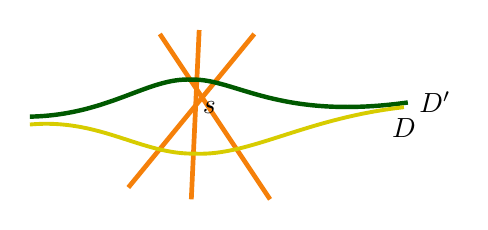
\begin{tikzpicture}[x=1cm,y=1cm]
\draw[orange!85!brown,line width=1.7pt] (-.85,1.05)--(.55,-1.05);
\draw[orange!85!brown,line width=1.7pt] (-.35,1.1)--(-.45,-1.05);
\draw[orange!85!brown,line width=1.7pt] (.35,1.05)--(-1.25,-.9);
\draw[green!35!black,line width=1.6pt] (-2.5,0) .. controls (-1.5,.02) and (-1,.5) .. (-.45,.47) .. controls (.1,.49) and (.65,-.05) .. (2.3,.18) node[right,black] {$D'$};
\draw[yellow!65!olive,line width=1.4pt] (-2.5,-.1) .. controls (-1.6,-.02) and (-1.1,-.48) .. (-.4,-.47) .. controls (.3,-.5) and (1,-.02) .. (2.25,.12) node[below,black] {$D$};
\node at (-.22,.12) {$\unsure{s}$};
\end{tikzpicture}}
% E: text|left middle beside figure continuing below|Ici il n'y a pas d'ambiguïté
Ici, il n'y a pas d'ambiguïté possible sur les arcs le long desquels faire le recollement, \unsure{ni} \unsure{par|sur} l'interprétation des \unsure{arcs de spécialisation non plus} (il faudrait du vice pour \unsure{l'antipodisme} pour recoller!). Ici, il est très tentant de remplacer encore $\Delta_D,\Delta_{D'}$ par $\Delta_D^*,\Delta_{D'}^*$ déduits en balayant les bords jusqu'au point $s$ ``critique'' qui nous intéresse, \deleted{\unsure{pour}} de recoller.
% E: margin note|left margin at il faudrait du vice|exclamation and vertical emphasis
\margin{!\ \figure{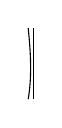
\begin{tikzpicture}[baseline]\draw (0,0)..controls(.05,.3)and(.03,.6)..(0,.9);\draw(.07,0)--(.07,.9);\end{tikzpicture}}}
% E: insertion|left lower middle above à partir|Revenant aux figures symétriques
\inserted{\unsure{Revenant} aux figures symétriques}
% E: text|bottom left continuing right|à partir de la position semi-stable
(à partir de la position semi-stable intermédiaire) on a à priori $8$ possibilités de recollement, suivant \deleted{les \unsure{quatre}} quatre choix d'\unsure{éléments} dans $\{a,a'\}\times\{b,b'\}$, puis le choix d'orientation pour recoller $\alpha\in\{a,a'\}$ avec $\beta\in\{b,b'\}$. Mais déjà le choix d'un couple $(a,b')$ ou $(b,a')$ est exclu, à cause de la nécessaire symétrie temporelle. Donc il reste deux couples $(a,b),(a',b')$, et pour chacun choix parmi les deux possibilités de recollage --- transport parallèle, ou l'opposé. Mais modulo \deleted{\unsure{application}} transformation, par antipodismes de part et d'autre (qui ne \unsure{change pas} la surface $\mathcal X$ \unsure{obtenue par recollement} \unsure{sans $D$ car disparu de la donnée|sans $D$ car disponible en la donnée}) \unsure{cas|des} $(a,b)$.
% E: drawing|top right cancelled pair|a a' and adjacent pencil outline
\deleted{\figure{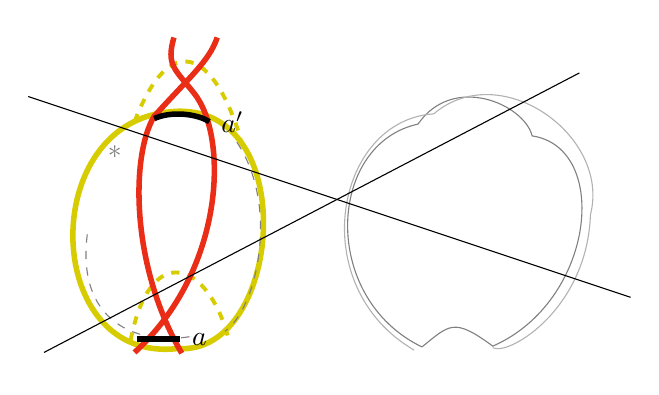
\begin{tikzpicture}[x=1cm,y=1cm]
\draw[yellow!65!olive,line width=2pt] (0,0) .. controls (-1.7,-.2) and (-1.8,2.8) .. (-.15,3) .. controls (1.6,3.25) and (1.35,-.1) .. (0,0);
\draw[yellow!65!olive,dashed,line width=1.4pt] (-.55,2.88)..controls(-.1,4.05)and(.45,3.8)..(.8,2.66);
\draw[yellow!65!olive,dashed,line width=1.4pt] (-.6,.1)..controls(-.35,1.4)and(.4,1.1)..(.65,.1);
\draw[gray,dashed] (-1.15,1.45)..controls(-1.3,.25)and(-.4,.02)..(.25,.17);
\draw[gray,dashed] (.75,2.62)..controls(1.3,1.8)and(1,.5)..(.6,.22);
\draw[red!65!brown,line width=2pt] (-.55,-.05)..controls(.6,1)and(.65,2.7)..(.2,3.25)..controls(-.04,3.55)and(-.15,3.6)..(-.05,3.95);
\draw[red!65!brown,line width=2pt] (.05,-.06)..controls(-.6,1.05)and(-.6,2.45)..(-.3,2.95)..controls(.15,3.45)and(.4,3.65)..(.5,3.95);
\draw[line width=2pt] (-.3,2.92)..controls(-.08,3.02)and(.25,2.98)..(.4,2.88) node[right] {$a'$};
\draw[line width=2pt] (-.52,.12)--(.03,.12) node[right] {$a$};
\node[gray] at (-.8,2.5) {$\unsure{*}$};
\draw[gray] (3.1,.02)..controls(1.8,.65)and(1.9,2.6)..(3.05,2.85)..controls(3.5,3.5)and(4.4,3.1)..(4.5,2.7)..controls(5.5,2.55)and(5.3,.6)..(4,.03)..controls(3.5,.4)and(3.45,.3)..(3.1,.02);
\draw[gray!60] (3,-.02)..controls(1.6,.8)and(2,2.9)..(3.25,2.98)..controls(4.1,3.7)and(5.5,2.7)..(5.24,1.7)..controls(5.2,.5)and(4.2,-.1)..(4,.01);
\draw (-1.9,3.2)--(5.75,.65);\draw(-1.7,-.05)--(5.1,3.5);
\end{tikzpicture}}}
% E: drawing|right middle|four arcs a a' b b'
\figure{\begin{tikzpicture}[x=1cm,y=1cm]
\draw[green!30!black,line width=1.6pt] (-.5,3.25)..controls(-2.4,2.85)and(-2.1,.25)..(-.55,.13);
\draw[green!30!black,line width=1.6pt] (.52,3.23)..controls(2.2,2.8)and(2.25,.35)..(.5,.16);
\draw[red!70!brown,line width=2pt] (-.45,-.28)..controls(.75,.5)and(.7,2.85)..(-.3,3.63);
\draw[red!70!brown,line width=2pt] (.55,-.3)..controls(-.7,.6)and(-.6,2.95)..(.48,3.62);
\draw[yellow!60!olive,line width=1.5pt] (-.56,3.28)..controls(-.58,2.71)and(.54,2.61)..(.6,3.25);
\draw[green!30!black,line width=2.3pt] (-.56,3.3)..controls(-.38,3.86)and(.44,3.84)..(.57,3.36);
\draw[black!75!brown,line width=2.3pt] (-.3,2.91)..controls(-.1,2.8)and(.28,2.8)..(.4,2.94);
\draw[yellow!60!olive,line width=1.5pt] (-.55,.14)..controls(-.5,-.4)and(.45,-.45)..(.5,.13);
\draw[green!30!black,line width=2.3pt] (-.5,.18)..controls(-.42,.75)and(.4,.75)..(.55,.2);
\draw[black!75!brown,line width=2.3pt] (-.32,-.18)..controls(-.05,-.27)and(.23,-.3)..(.38,-.22);
\node at (0,3.89) {$b^{\deleted{\unsure{*}}}$};
\node at (.02,2.66) {$a'$};\node at (-.05,.82) {$b'$};
\node at (.61,.69) {$\deleted{\unsure{b}}$};\node at (.05,-.48) {$a$};
\end{tikzpicture}}
\scanpage{73}
\mspage{72}
% E: drawing|lower left upper row|two vertices on a line and transverse rays
\figure{\begin{tikzpicture}[x=1cm,y=1cm]
\draw[gray,line width=1pt] (-2,0)--(2,.25);
\fill(-.45,.1)circle(1.5pt);\fill(1.15,.2)circle(1.5pt);
\draw[gray] (-.7,.72)--(-.45,.1)--(.05,.85);\draw[gray] (-.43,.67)--(-.42,-.25);
\draw[gray] (.45,-.15)--(.45,.85);
\draw[gray] (.85,.75)--(1.15,.2)--(1.45,-.35);\draw[gray] (1.5,.88)--(1.15,.2)--(.91,-.37);\draw[gray](1.18,.9)--(1.1,-.37);
\end{tikzpicture}}
% E: display|beneath two-vertex drawing written inverted|n-1 minus two terms
\[ (n-1)-(\unsure{\nu|\mu}-1)-(\unsure{\nu'|\mu'}-1) \qquad n-\nu \]
% E: drawing|lower middle upper row|two sloping parallel segments and dots
\figure{\begin{tikzpicture}[x=1cm,y=1cm]
\draw[gray] (-1.5,0)--(-.65,1.9)--(1.55,1.73)--(1.56,.82);
\draw[gray!60] (1.6,1.69)--(1.9,.35);
\draw[gray] (-1.4,.05)--(1.55,.28);\draw[gray](-2,.21)--(.98,.38);\draw[gray](-2,.25)--(-1.4,.3);
\fill(.22,1.82)circle(1.3pt);\fill(.48,1.8)circle(1.3pt);\fill(-.5,.35)circle(1.4pt);
\foreach \x in {-1.4,-.8,-.2,.4,1}{\draw[gray!65](\x+.4,.4)--(\x,-.55);}
\end{tikzpicture}}
% E: drawing|lower right upper row|point with six radial strokes
\figure{\begin{tikzpicture}[x=1cm,y=1cm]
\draw[gray](-.05,-1)--(.04,1.15);\draw[gray](-.9,.95)..controls(-.6,.5)and(.3,-.3)..(.65,-.68);\draw[gray!65](-.85,-.55)--(.75,.65);\draw[gray](-.8,.9)--(.55,-.65);\fill(0,0)circle(1.2pt);
\end{tikzpicture}}
% E: drawing|bottom left pencil construction|one vertex transverse line and arrow
\figure{\begin{tikzpicture}[x=1cm,y=1cm]
\draw[gray,line width=.8pt,->](-1.4,-.15)--(1.3,.35);\draw[gray](-.55,1.2)--(.32,-1.2);\draw[gray!60](.72,1.05)..controls(.6,.68)and(.5,.75)..(.35,.58);\fill(-.13,.08)circle(1.4pt);
\end{tikzpicture}}
% E: drawing|bottom centre pencil construction|three crossing directions
\figure{\begin{tikzpicture}[x=1cm,y=1cm]
\draw[gray](-1.55,-.12)--(1.2,.15);\draw[gray](0,1.3)--(.06,-1.1);\draw[gray](-1.8,1.3)--(1.1,-.75);\draw[gray!70](-.9,.62)..controls(.1,-.05)and(.9,-.5)..(1.3,-1.08);
\end{tikzpicture}}
% E: drawing|bottom centre right|polygon fan with doubled bent strip
\figure{\begin{tikzpicture}[x=1cm,y=1cm]
\draw[gray!75] (-1.42,-.55)--(-1.25,1.15)--(.15,2.15)--(1.75,1.55)--(2.02,-.16)--(1.15,-1.35)--(-.7,-1.35)--cycle;
\draw[gray!65](-1.3,-.25)--(2,-.05);\draw[gray!65](-1.3,-.12)--(2,.04);
\draw[gray!70](-.7,-1.35)--(1.75,1.55);\draw[gray!70](1.15,-1.35)--(-.7,2.2);
\fill(.48,-.08)circle(1.5pt);
\draw[gray!65](-1.5,1.2)--(2.7,1.45);\draw[gray!65](-1.45,1.38)--(2.8,1.58);
\foreach \x/\y in {-1/.85,.3/1.5,1.35/1.18}{
\draw[gray!65](\x-.45,\y+.65)--(\x+.45,\y-.65);\draw[gray!65](\x-.55,\y-.45)--(\x+.55,\y+.6);\draw[gray!65](\x-.65,\y+.08)--(\x+.65,\y-.08);\draw[gray!65](\x+.05,\y+.8)--(\x-.05,\y-.6);
}
\draw[black!75,line width=1.4pt](-1.32,.62)--(.28,1.84)--(1.99,1.29)--(1.63,.57)--(.28,1.27)--(-.83,.48);
\draw[gray,line width=.8pt](-1.28,.69)--(.34,1.91)--(2.05,1.34)--(1.69,.54)--(.23,1.2)--(-.89,.43);
\draw[gray!65](1.99,1.29)..controls(2.45,1.42)and(2.7,1.63)..(3.08,1.85);
\draw[gray!65](-1.36,-.72)..controls(-.8,-1.5)and(-.37,-1.5)..(-.08,-1.8);\draw[gray!65](.6,-1.85)--(2.2,-1.2);
\end{tikzpicture}}
% E: text|bottom printed block inverted|JOB CRAY2
{\ttfamily
/*JOB=CRAY2,ACCT=*********,ALL=M06,MSGL=N\hfill J0424CNU\par
// JOB MSGLEVEL=(1,1),MSGCLASS=A\par
// EXEC PGM=IEFBR14\par}
% E: display|bottom manuscript inverted above sigma sequence|N=4n
\[N=4n\]
% E: display|bottom manuscript inverted first line|sigma0 sigma1 dash sigmaN-1
\[\sigma_0\sigma_1\mathbin{-}\sigma_{N-1}\ \big|\ \sigma_N=\sigma_0\qquad \sigma_i^2=1\]
% E: display|bottom manuscript inverted second line|rho1 sigma0 sigma1
\[\rho_1=\sigma_0\sigma_1\quad \rho_2=\sigma_1\sigma_2\quad\cdots\quad \rho_N=\sigma_{N-1}\sigma_N=\sigma_{N-1}\sigma_0\]
% E: text|bottom manuscript inverted right|rho_i squared one
$\rho_i^2=1$ i.e. deux $\sigma_i$ consécutifs (circulairement) commutent
% E: display|bottom manuscript inverted final line|rho1 rho2
\[\rho_1\rho_2=\sigma_0\sigma_2\qquad\rho_2\rho_3=\]
\scanpage{74}
\mspage{73}
% E: drawing|top left|oriented rives and crossed coloured strands
\figure{\begin{tikzpicture}[x=1cm,y=1cm]
\foreach \x in {-2.4,-1.85,-1.3,-.65,.1,.8,1.4,2}{\draw[yellow!65!orange,line width=1.2pt](\x,.1)--(\x+.8,1.55);}
\foreach \x in {-2.4,-1.55,-.65,.4,1.25,1.85}{\draw[green!35!black,line width=1.4pt](\x,0)--(\x+.95,-1.7);}
\draw[red!70!brown,line width=2.1pt](-1.15,1)--(.25,-1.55);\draw[red!70!brown,line width=2.1pt](.05,1.2)--(-1.6,-1.25);
\draw[green!30!black,line width=2pt,<-](-2.55,.82)--(2.5,.8);\node at(-2.45,1.05){$\omega_{D'}$};
\draw[yellow!65!olive,line width=1.7pt,->](-2.6,-.74)--(2.2,-.64) node[right,black]{$\omega_D$};
\draw[green!30!black,dashed,line width=2pt](-2.6,.1)--(1.65,.2);\draw[yellow!65!olive,dashed,line width=1.7pt](-2.55,-.02)--(1.75,.04);
\draw[line width=3pt](-.89,.12)--(-.42,.16);\draw[line width=2pt](-.9,-.04)--(-.36,-.03);
\draw[->](2.28,1.31)arc(-55:230:.18);\node at(2.76,1.37){$\omega_F$};
\draw[->](2.06,-1.68)arc(-90:190:.18);\node at(2.62,-1.73){$\omega_{F'}$};
\end{tikzpicture}}
% E: drawing|upper middle|alternative a' b' and reversed hatching
\figure{\begin{tikzpicture}[x=1cm,y=1cm]
\draw[gray](-2.45,1.55)..controls(-2.7,1.8)and(-2.7,1.2)..(-2.7,.8)--(-2.7,-1.4)..controls(-2.7,-1.6)and(-2.5,-1.6)..(-2.43,-1.6);
\node at(-1.8,.2){ou};\node at(-1.8,-1){$(a',b')$};
\foreach \x in {-.3,.4,1.2,1.8}{\draw[green!30!black,line width=1.3pt](\x,0)--(\x+.82,1.5);}
\foreach \x in {-.2,.4,.9,1.5,2}{\draw[yellow!65!olive,line width=1.4pt](\x,-.27)--(\x+.7,-1.75);}
\draw[red!70!brown,line width=2pt](.6,1.1)--(1.45,-1.6);\draw[red!70!brown,line width=2pt](1.55,1.1)--(.35,-1.45);
\draw[green!30!black,line width=1.8pt](-.4,.82)--(2.35,.88);
\draw[green!30!black,dashed,line width=1.8pt](-.35,0)--(2.5,.05);\draw[yellow!65!olive,dashed,line width=1.6pt](-.25,-.2)--(2.42,-.2);\fill(.91,-.02)circle(2pt);
\draw[gray!65](-.45,.95)--(.98,-1.3);\draw[gray!60](-2.5,-.13)--(2.1,-.1);
\end{tikzpicture}}
% E: text|upper right|car un peu vicieux
(car un peu vicieux, et sans intérêt!)
% E: text|left below figures|Cas a b de prolongation des rives
\deleted{\unsure{4)}} Cas $(a,b)$ \deleted{c'est le cas} de \uline{prolongation des rives}.
% E: text|left middle|1 On choisit comme recollement
1) On choisit comme recollement le transport parallèle. On trouve un $\mathcal X$ \deleted{avec} $\varphi:\mathcal X\longrightarrow X$ qui est une immersion.

Dans $\mathcal X$, on a un graphe \unsure{top.} $K$, et les faces de $(\mathcal X,K)$ correspondent aux p.r. stables \unsure{\&} \deleted{\unsure{on a un}} On a un $L=\varphi^{-1}(X_1)$, qui matérialise la corr. entre faces et p.r. stables --- en prolongeant chaque face $F$ par la face $\widetilde F$ obtenue en la ``renflant'' aux pts \deleted{qui} ``critiques'' de $S_K$ i.e. les pts de $K\cap S(L)$.
% E: text|right middle|NB Ici en partant d'une orientation
\uline{NB} Ici, en partant d'une orientation $\omega_F$ de $F=\Delta_D^*$, c.à.d. $\omega_D$ orientation de $D$, passant à l'orientation $\omega'$ de $\Delta_{D'}^*$ déduite par transport via le recollement, et \unsure{une} orientation $\omega_{D'}$ de $D'$, on constate encore que c'est l'\uline{opposée} de celle obtenue par transport parallèle!
% E: margin note|beside NB|D in Delta and D' in Delta'
\margin{\diagram{\begin{tikzcd}[row sep=small]
\unsure{D\subset\Delta_D^*|D_i\Delta_D^*}\arrow[d,bend left=30,"\text{pour}"]\\
D'\subset\Delta_{D'}^*
\end{tikzcd}}}
% E: margin note|right margin at opposite orientation|L'ennui c'est que
\margin{L'ennui, c'est que les circuits sont \unsure{stériles|triviaux}. On n'obtient \unsure{rien} par les bons circuits supersinguliers!}
% E: text|bottom right|2 Recollement par l'iso opposé
2) Recollement par l'iso. \inserted{$a\simeq b$} opposé au transport parallèle. Cette fois, c'est au niveau de la transition $\underline\omega_F\mathbin{-}\underline\omega_{F'}$, interprétée comme $\underline\omega_D\mathbin{-}\underline\omega_{D'}$, qu'on obtient le transport parallèle. Contrairement à ce que je croyais \inserted{\unsure{avoir vu}} on trouve les bons circuits autour des positions supersingulières
\scanpage{75}
\mspage{74}
% E: text|upper left|Mais les circuits plus généraux
Mais les circuits plus généraux restent mystérieux pour moi --- je ne sais s'ils sont \unsure{bidons|stables}!
% E: text|left upper middle|Ces deux procédés correspondent
Ces deux procédés correspondent à la $=$ structure polygonale sur l'un des arcs de spécialisation \inserted{(= transition)} pour une p.r. stable $D$ --- mais il y a une autre structure polygonale, due au fait que les \deleted{\unsure{arcs des}} arcs de spécialisation \uline{sur $D$} (au lieu de $\widetilde D$) sont mutuellement disjoints, donc on peut prendre la structure polygonale correspondante, dont la réalisation top. est \unsure{cert.} $D$ lui-$=$. L'ennui, c'est que cette fois on a un polygone \deleted{\unsure{d'ordre double}} \inserted{d'ordre $n$} \unsure{en $2n$|au $2n$}, dont la signification géométrique \unsure{du disque-polygone|du disque recollé} correspondant n'est pas \unsure{clair|claire}. Mais peut-être est-ce une indication pour obtenir \uline{simultanément} \uline{de deux façons} antipodiques les disques $\Delta_D^*,\Delta_{D'}^*$, de façon à obtenir un ruban de Möbius peut-être?
% E: text|top right continuing beside drawing|L'idée maintenant c'est de
L'idée maintenant c'est de prendre le découpage de $X$ suivant la partie commune de $D$ et $D'$ (cf figure)
% E: drawing|upper right|lens bounded by two coloured curves crossed by red lines
\figure{\begin{tikzpicture}[x=1cm,y=1cm]
\draw[red!70!brown,line width=2pt](-.15,1.35)--(.75,-1.25);\draw[red!70!brown,line width=2pt](.8,1.45)--(-.6,-1.35);
\draw[green!30!black,line width=2pt](-3,.02)--(-1.1,.1)..controls(-.6,.85)and(.85,1)..(1.6,-.1)--(2.85,-.05);
\draw[yellow!65!olive,line width=2pt](-3,-.06)--(-1.1,.03)..controls(-.7,-1)and(.85,-.95)..(1.6,-.15)--(2.95,-.16);
\draw[black!80!brown,dashed,line width=2.4pt](-.85,.06)--(1.5,-.02);
\end{tikzpicture}}
% E: text|right middle|Ça donne donc un ruban de Möbius
Ça donne donc un ruban de Möbius, \deleted{\unsure{qui se trouve}} \inserted{découpé par la ligne} pointillée en une bande rectangulaire. On prend le revêtement \deleted{\unsure{de}} \inserted{des orientations \unsure{d'}} d'ordre $2$ du ruban de Möbius, \inserted{(\uline{twisté} par $\underline\omega(D)$?)} qui est formé de deux rectangles recollés en $2$ paires d'arêtes. Sauf erreur, c'est l'identification \deleted{\unsure{de}} simultanée de \deleted{$a'$}\inserted{$a$} avec $b$, \unsure{et} \deleted{$a$}\inserted{$a'$} avec $b'$, suivant le transport parallèle. Mais ce qu'on obtient, en faisant tous ces recollements pour l'\unsure{ens.} de tous les $\Delta_D^*$ est-elle bien la surface cellulaire obtenue par le graphe $\unsure{\Gamma|\mathcal G}$ et sa structure de polygonalisation et de transport?) obtenue
\scanpage{76}
\mspage{75}
% E: text|upper left|par recollement des polygones d'arêtes
par recollement \uline{des} polygones \uline{d'arêtes}, \unsure{en $2n$|au $2n$}? \deleted{Cette} La première ne serait-elle pas plutôt un revêtement d'ordre deux de la seconde, ramifiée en chacun des pts du centre --- en effet, on sait \deleted{\unsure{apparemment}} \inserted{que les} antipodismes des $\Delta_D^*$ sont compatibles avec les identifications, --- par passage au quotient, cela donnera \unsure{sûrement} la carte cellulaire envisagée\unsure{\ldots} On peut alors, \deleted{qui} \unsure{pour} \deleted{\unsure{une seconde}} interpréter la nouvelle carte comme associée à un graphe \inserted{(\unsure{polygonalement})} dont les sommets sont les p.r. stables, que pour deux p.r. $D,D'$ adjacentes, on va maintenant envisager \uline{deux} flèches orientées entre eux, savoir $a_D:D\longrightarrow D'$ (\unsure{de le bord|de bords} $a$ vers $b'$) et $a_{D'}:D'\longrightarrow D$ (\unsure{de l'autre|de bords} $b$ vers $a'$), munies chacune d'une orientation --- le balayage de $D$ vers $D'$, et de $D'$ vers $D$, qu'on \unsure{désidentifie}.
% E: text|upper right|Maintnt les arcs de transition
\unsure{Maintnt|Maintt}, les arcs de transition (ancien style) pour $D$ i.e. sur $\partial\Delta_D$, sont les arcs de spécialisation \uline{et leurs antipodiques}, organisés en polygône de la façon habituelle. On considère que par l'un ou par l'autre, on va d'\unsure{une vers une} position rel. adjacentes.
% E: text|right middle|La surface Xcal obtenue
La surface $\mathcal X$ obtenue, immergée dans $X$ par une immersion, \unsure{l'image inverse} \inserted{$L$} de $X_1$ \deleted{est} donne lieu à \deleted{une} l'interprétation habituelle de la p.r. (stable) associée à une face de $(\mathcal X,K)$.
% E: text|bottom right heading|Description combinatoire
Description combinatoire
% E: display|bottom right|1 graphe Gamma sommets and arêtes orientées
\diagram{\(\begin{array}{ll}
1)\ \text{graphe }\Gamma & \left\{\begin{array}{l}
\text{sommets: p.r. stables }D\\
\text{Arêtes orientées: paires }(D,a),\ a\text{ un}\\
\qquad\text{arc de transition, sur }\underline D\\
\deleted{\text{\unsure{où}}}\qquad\text{(de spécialisation,}\ \text{ou antipodique}\\
\qquad\text{d'un tel)}
\end{array}\right.
\end{array}\)}
